\RequirePackage{tikz}
\documentclass[pdflatex,sn-mathphys]{sn-jnl}
\usetikzlibrary{positioning,arrows.meta,shapes.geometric,fit}

\usepackage[T1]{fontenc}
\usepackage{graphicx}
\usepackage{array,longtable}
\usepackage{mathtools}
\usepackage{amssymb}
\usepackage{float}
\usepackage{subcaption}
\usepackage{algorithm}
\usepackage{algpseudocode}
\usepackage{newtxtext,newtxmath}
\usepackage{pifont}
\usepackage{xurl}
\newcommand{\cmark}{\ding{51}}
\newcommand{\xmark}{\ding{55}}
\newcommand{\pmark}{$\circ$}

\graphicspath{{./}{figures/}}
\jyear{2026}

\theoremstyle{thmstyleone}
\newtheorem{theorem}{Theorem}
\newtheorem{proposition}[theorem]{Proposition}
\newtheorem{corollary}[theorem]{Corollary}
\newtheorem{appproposition}{Proposition}
\renewcommand{\theappproposition}{A\arabic{appproposition}}
\theoremstyle{thmstyletwo}
\newtheorem{remark}{Remark}
\theoremstyle{thmstylethree}
\newtheorem{definition}{Definition}

\newcommand{\Acc}{\mathrm{Acc}}
\newcommand{\BalAcc}{\mathrm{BalAcc}}
\newcommand{\AUDC}{\mathrm{AUDC}}
\newcommand{\MRR}{\mathrm{MRR}}
\newcommand{\aMRR}{\mathrm{aMRR}}
\newcommand{\etamax}{\eta_{\max}}
\newcommand{\etaknee}{\eta_{\mathrm{knee}}}

\setcounter{topnumber}{4}
\setcounter{bottomnumber}{4}
\setcounter{totalnumber}{8}
\renewcommand{\topfraction}{0.95}
\renewcommand{\bottomfraction}{0.95}
\renewcommand{\textfraction}{0.05}
\renewcommand{\floatpagefraction}{0.75}

\setlength{\textfloatsep}{8pt plus 2pt minus 2pt}
\setlength{\floatsep}{6pt plus 2pt minus 2pt}
\setlength{\intextsep}{6pt plus 2pt minus 2pt}
\setlength{\abovecaptionskip}{3pt}
\setlength{\belowcaptionskip}{2pt}

\raggedbottom

\begin{document}

\title[TabStress: Nonparametric Robustness Profiling of Tabular Classifiers]{TabStress: Nonparametric Robustness Profiling of Tabular Classifiers under Controlled Data Corruption}

\author[1]{\fnm{Devarsh} \sur{Patel}}\email{devarsh.patel2024@vitstudent.ac.in}
\author*[1]{\fnm{Shashank Mouli} \sur{Satapathy}}\email{shashankmouli.s@vit.ac.in}

\affil*[1]{\orgdiv{School of Computer Science and Engineering}, \orgname{Vellore Institute of Technology}, \orgaddress{\city{Vellore}, \postcode{632014}, \state{Tamil Nadu}, \country{India}}}

\abstract{Tabular benchmarks rank classifiers by clean accuracy, yet deployed models meet noisy labels, corrupted features and missing values. TabStress treats robustness as a response curve: accuracy across eleven intensities of controlled corruption, summarized by absolute and relative endurance scores and tested across datasets. Six classical families are evaluated on twenty OpenML datasets under label noise, Gaussian and categorical-aware feature noise, and MCAR, MAR and MNAR missingness (stochastic, not adversarial). Protocol~A measures the robustness of a learning procedure trained on corrupted data; Protocol~B measures a trained model scored on corrupted inputs. Balanced area under the degradation curve ($\AUDC_{\mathrm{bal}}$) is the primary score, computed over 22{,}280 Protocol~A cells and 25{,}740 Protocol~B cells. Fifteen confirmatory rank tests reject equal performance after joint Holm adjustment. Clean accuracy does not reliably predict robustness: the most accurate clean model also has the highest balanced AUDC in only 46\% of dataset--condition blocks, and rankings depend on corruption mechanism, metric, training budget and protocol. Under a matched 100-round boosting budget LightGBM leads on balanced AUDC under most conditions, but this lead is coupled to the budget: with CatBoost at its library default of 1{,}000 rounds, CatBoost leads under Gaussian feature noise. In an exploratory, Protocol~B-only check of one in-context model (TabICL) under a constrained inference budget (four estimators, 3{,}000 context rows), higher clean accuracy did not yield higher retention under inference-time corruption. Endurance scores replicate across seeds. These are controlled-benchmark findings, not direct evidence of real-world robustness.}

\keywords{tabular classification, robustness evaluation, data corruption, label noise, missing data, average-case stochastic corruption}

\maketitle

%% ===========================================================================
\section{Introduction}\label{sec:intro}

\subsection{Motivation}\label{sec:intro:motivation}

Grinsztajn et al.~\cite{grinsztajn2022tree} and McElfresh et al.~\cite{mcelfresh2023when} compared tabular learners on clean data, and Borisov et al.~\cite{borisov2024deep} surveyed deep models for tables. Tuned gradient-boosted trees remain hard to beat on medium-sized tables, and the reasons are increasingly well understood. A deployed classifier, however, rarely meets the data it was benchmarked on. Labels come from annotators who disagree, measurement channels drift, and fields go missing in transmission or are never recorded~\cite{sambasivan2021everyone}. The accuracy printed in a model-selection table describes none of these operating conditions.

\subsection{Problem and research gap}\label{sec:intro:gap}

A clean benchmark observes each model at one point, corruption level zero. A single additional evaluation at a chosen corruption level does not repair this, because two models with the same clean accuracy can separate at moderate corruption and meet again at heavy corruption, and the choice of level then decides the conclusion. Robustness is better represented as a continuous \emph{response curve}: accuracy as a function of the intensity of a controlled corruption. Corruption benchmarks in computer vision~\cite{hendrycks2019benchmarking} and sensor systems~\cite{mena2025multisensor} summarize such curves; Zhu and Wu~\cite{zhu2004class}, Nettleton et al.~\cite{nettleton2010study} and S\'aez et al.~\cite{saez2015evaluating} varied noise levels for earlier learners. These components exist separately, and what remains open is a single tabular evaluation that joins them (Section~\ref{sec:related:gap}).

Two design questions must be resolved before such an evaluation measures what practitioners require. First, \emph{when} is the corruption introduced? If training and evaluation data are corrupted together, the learner adapts to the corruption at every intensity, measuring the robustness of the \emph{learning procedure} under a persistently degraded process (Protocol~A). If a model is trained on clean historical data and then scored on corrupted inputs, the curve measures the robustness of a \emph{trained model} to deteriorating evaluation inputs at inference (Protocol~B). The two estimands can rank models differently, and we report both. Second, \emph{which score} carries the conclusion? On imbalanced data accuracy can be retained merely by drifting towards the majority class, and a ratio to clean accuracy can artificially reward classifiers that had little accuracy to lose. We therefore formalize primary confirmatory metrics and baseline-adjusted sensitivity scores within a structured family-wise error control framework (Section~\ref{sec:method:stats}).

\subsection{Research questions}\label{sec:intro:rq}

\begin{description}
\item[RQ1] Does clean-data performance predict robustness under controlled corruption?
\item[RQ2] How do robustness rankings of tabular model families depend on the corruption mechanism, the robustness metric, the model configuration and the evaluation protocol?
\item[RQ3] Is a single inflection point (a ``knee'') of a degradation trajectory identifiable from a curve sampled at eleven intensities, as knee and elbow detectors~\cite{satopaa2011finding,salvador2004determining} presuppose? (A methodological audit with a negative answer; see Section~\ref{sec:res:knee}.)
\end{description}

\subsection{Contributions}\label{sec:intro:contrib}

We introduce TabStress, a standardized open-source empirical stress-testing suite for tabular classifiers, evaluating degradation profiles, cross-family endurance rankings and deployment trade-offs across more than 48{,}000 evaluation cells under two protocols and three configuration regimes. No single component of the framework is claimed as new; the contribution is the combination of these components in one controlled tabular evaluation:
\begin{enumerate}
\item \emph{Dual-protocol corruption-response evaluation framework.} Two protocols share one corruption engine, one set of folds and one set of seeds: corruption-aware training robustness (Protocol~A) and deployment inference robustness (Protocol~B). The engine spans nine stochastic operators across label noise, continuous Gaussian and nominal categorical perturbations, and MCAR, MAR, and MNAR missingness, with both median imputation and native tree handling (Section~\ref{sec:problem}).
\item \emph{Dual absolute and relative endurance measures with explicit baselines.} Balanced AUDC is the designated primary robustness measure, AUDC the capacity-weighted absolute measure, and MRR the relative retention score; an adjusted retention ratio (aMRR) removes the majority-class baseline to prevent weak models from appearing robust (Section~\ref{sec:problem:metrics}).
\item \emph{Statistically controlled cross-dataset evaluation methodology.} A designated confirmatory hypothesis family with joint Holm error control, Friedman and Iman--Davenport omnibus tests, Nemenyi critical difference, and Holm-adjusted pairwise Wilcoxon tests replicated across three seeds (Section~\ref{sec:method:stats}).
\item \emph{Methodological audit of trajectory knees.} We audit whether a degradation trajectory has an identifiable knee and find that, at the sampling resolution of a standard sweep, it is not reliably identifiable: the maximum-curvature knee $\etaknee$ is forced into the interior by the spline boundary conditions, unstable across seeds, and reports false knees on knee-free trajectories. This is a cautionary negative result for curve-based robustness reporting, not a proposed robustness measure; the knee is not used in any ranking (Section~\ref{sec:res:knee}).
\item \emph{Evidence on factors governing robustness rankings.} On twenty OpenML datasets, six classical model families, and one pretrained model, an exploratory TabICL baseline under a constrained inference budget, we find that clean accuracy does not reliably predict robustness, that rankings depend on corruption mechanism, metric, configuration and protocol, and that no single family dominates all conditions (Section~\ref{sec:results}).
\end{enumerate}

These are comparative baselines under controlled, synthetic and stochastic corruption on twenty public datasets. They are not guarantees for uncurated production feeds, and the rankings reflect standardized configurations (such as the matched 100-round boosting budget) rather than immutable architectural superiority.

The remainder of the article is organized as follows. Section~\ref{sec:related} reviews related work and states the gap. Section~\ref{sec:problem} formulates the problem, the corruption taxonomy, the robustness metrics and the knee. Section~\ref{sec:method} describes the TabStress methodology and the experimental and statistical protocol. Section~\ref{sec:results} reports the results, Section~\ref{sec:discussion} discusses them, Section~\ref{sec:threats} examines threats to validity and Section~\ref{sec:conclusion} concludes.

%% ===========================================================================
\section{Related Work}\label{sec:related}

\subsection{Tabular benchmarking}\label{sec:related:benchmarks}

Comparative studies of supervised learning on tabular data are organized around performance at a single operating point: a model is configured, trained and scored on data whose labels and covariates are taken as given, and the resulting scalar enters a cross-dataset ranking. Grinsztajn et al.~\cite{grinsztajn2022tree} attributed the persistent advantage of gradient-boosted trees over deep networks to the irregularity of tabular target functions, the sensitivity of MLP-type architectures to uninformative features and the absence of rotational invariance. Under corruption that advantage is conditional: a clean-trained MLP leads under Gaussian noise (Section~\ref{sec:res:deploy}). McElfresh et al.~\cite{mcelfresh2023when} extended the comparison to many algorithms and datasets and related the residual differences to dataset meta-features, against deep baselines established by~\cite{gorishniy2021revisiting,borisov2024deep}. TabStress tests whether that clean ordering survives corruption (Section~\ref{sec:res:overall}). More recent benchmarks widen coverage without moving the operating point: TabArena~\cite{nick2025tabarena} maintains a living leaderboard in which pretrained tabular foundation models such as TabPFN~\cite{hollmann2023tabpfn,hollmann2025accurate} do best on small training sets, and an uncertainty benchmark of tabular foundation models~\cite{jos2026high} reports that high predictive performance does not imply reliable uncertainty, so a ranking on clean data says little about operational behavior.

\subsection{Label and feature corruption}\label{sec:related:corruption}

Fr\'enay and Verleysen~\cite{frenay2014classification} separate label noise that is independent of class and covariates from class-conditional noise and from noise that also depends on the covariates; our symmetric and class-conditional operators instantiate the first two categories. Zhu and Wu~\cite{zhu2004class} quantified the separate effects of class and attribute noise, Nettleton et al.~\cite{nettleton2010study} compared learners under several noise types, and S\'aez et al.~\cite{saez2015evaluating} proposed the equalized loss of accuracy, which judges a classifier on noisy data by performance and robustness together. Ghosh et al.~\cite{ghosh2017robustness} proved large-sample robustness of decision-tree learners to symmetric label noise, and Natarajan et al.~\cite{natarajan2013learning} showed that class-conditional noise translates the Bayes decision threshold. Surveys of learning with noisy labels~\cite{song2023learning} and confident learning~\cite{northcutt2021confident} concentrate on estimating, cleaning or tolerating the noise. Recent tabular work on noisy labels is likewise mostly corrective, for example noise-aware boosting~\cite{ye2026itboost}. Sweeps of the noise rate are typically run to answer one question, such as whether decision-tree learners tolerate symmetric noise better than support vector machines~\cite{ghosh2017robustness}, and report accuracy at each level without an endurance score or a cross-dataset test. Feature corruption in tabular data is usually studied as measurement error proportional to the dispersion of an attribute; categorical attributes require operators that keep values valid, a point we return to in Section~\ref{sec:problem:taxonomy}.

\subsection{Missing-data robustness}\label{sec:related:missing}

The distinction between data missing completely at random, at random and not at random~\cite{rubin1976inference} governs what any analysis of incomplete data can recover~\cite{little2019statistical}. For prediction, impute-then-predict pipelines can be consistent, and the best handling depends on the learner and the mechanism~\cite{josse2024consistency,lemorvan2021whats}; benchmarks on health databases compare imputation with native handling at the missingness rates observed in the data~\cite{perezlebel2022benchmarking}, and decision trees have been compared under several missing-data techniques~\cite{twala2008good}. In replicated benchmarks, unconstrained protocol choices such as preprocessing, encoding and missing-value handling shift the fitted results~\cite{bischl2021openml,mcelfresh2023when}; under test-time missingness, tree ensembles remain highly competitive against neural representations~\cite{lemorvan2021whats,mcelfresh2023when}; and feature degradation impacts complex tabular learners even when discriminative attributes are preserved~\cite{borisov2024deep,hollmann2023tabpfn}. Most robustness sweeps use MCAR masking, the least structured mechanism. TabStress adds rank-based MAR and self-masking MNAR operators and compares median imputation with the native missing-value routing of the tree libraries under each.

\subsection{Robustness curves and data-centric evaluation}\label{sec:related:curves}

Corruption benchmarks in computer vision summarize a model's errors over several severities of each corruption by the mean corruption error (mCE) and its relative version~\cite{hendrycks2019benchmarking}; similarly, sensor-failure evaluations assess relative performance retention under corruptions across multiple measurement domains~\cite{mena2025multisensor}. Robustness curves, which plot performance against perturbation size instead of reporting a single score, have been advocated for adversarial perturbations~\cite{gopfert2020adversarial}, and conclusions drawn from a fixed corruption catalogue depend on how close the training augmentations are to it~\cite{mintun2021interaction}. Stress tests probe trained models with shifted or perturbed inputs and reveal that predictors with equal held-out accuracy can behave very differently~\cite{damour2022underspecification}. Distribution-shift benchmarks evaluate models under natural shifts: Recht et al.~\cite{recht2019imagenet} tested whether ImageNet classifiers generalize to a new test set, Taori et al.~\cite{taori2020measuring} measured robustness to natural shifts in image classification, and WILDS~\cite{koh2021wilds} collects in-the-wild shifts (see also~\cite{quinonero2009dataset}), including tabular shifts in TableShift~\cite{gardner2023tableshift}, where distribution shifts across demographic and temporal splits degrade tabular models systematically. Sensor-failure studies inject faults in specific domains: Mamun et al.~\cite{mamun2022designing} designed networks robust to sensor failure in mobile health, Rebelo de S\'a et al.~\cite{rebelodesa2019building} built prediction models for defective sensor data, and Mena et al.~\cite{mena2025multisensor} trained an earth-observation model to tolerate missing sensors. Data-centric evaluation makes the data rather than the model the object of study (DataPerf~\cite{mazumder2023dataperf}; Whang et al.~\cite{whang2023data}; Jain et al.~\cite{jain2020overview}); the closest tabular precedent for a sweep measures how six data-quality dimensions, polluted at increasing levels, affect many algorithms~\cite{mohammed2025effects}, and CleanML measures the effect of data cleaning on downstream models~\cite{li2021cleanml}. The methodological analogue of TabStress is the empirical analysis of learning curves~\cite{perlich2003tree} that treats error as a response along sample size and fits parametric trajectories; TabStress replaces sample size by corruption intensity and fits an interpolating natural cubic spline. Studies of empirical degradation also examine baseline-crossing severities~\cite{mena2025multisensor}, the point at which a model is no better than a naive predictor; such thresholds locate total failure, whereas the knee of TabStress locates the onset of accelerated deterioration, and the two are complementary. Our endurance scores are tabular counterparts of mCE and relative mCE: AUDC is the mean accuracy over the sweep and MRR its ratio to clean accuracy. The knee we compute should not be confused with the breakdown point of robust statistics~\cite{donoho1983notion}, the smallest contaminated fraction that can carry an estimator arbitrarily far; it is a descriptive feature of an empirical trajectory.

Statistical comparison of classifiers over several datasets follows Dem\v{s}ar~\cite{demsar2006statistical}: a Friedman rank test followed by the Nemenyi procedure, summarized in critical-difference diagrams and implemented, for example, in \texttt{autorank}~\cite{herbold2020autorank}. We add Holm-adjusted Wilcoxon tests, which separate more pairs than Nemenyi in 25 of 30 blocks. Benavoli et al.~\cite{benavoli2016should} showed that mean-rank post-hoc verdicts on a pair of algorithms depend on the other algorithms in the pool and recommended pairwise signed-rank tests with family-wise control; applied tabular studies use one or both~\cite{perezlebel2022benchmarking,borisov2024deep}. We report both and designate a confirmatory family.

\subsection{Research gap}\label{sec:related:gap}

Table~\ref{tab:comparison} places TabStress among the closest evaluations, and Table~\ref{tab:gaps} lists the gaps; each gap is the absence of evidence for a unified combination, not the absence of any study of degradation curves or corruption robustness. Three works are closest: Hendrycks and Dietterich~\cite{hendrycks2019benchmarking} summarized a few severities per corruption in vision, Mena et al.~\cite{mena2025multisensor} measured retention under sensor dropout, and Ghosh et al.~\cite{ghosh2017robustness} proved asymptotic tree robustness to symmetric label noise, yet at our sample sizes CART is last under that noise (Section~\ref{sec:res:label}). Each already provides part of the design: sweeps, integrated and relative scores, baseline-crossing severities, or theory under noise. Relative to them, TabStress adds, in terms of
(i)~\emph{evaluation design}, a move from isolated perturbations to continuous response curves across eleven controlled intensities and nine distinct corruption operators;
(ii)~\emph{estimands}, distinguishing the robustness of a learning procedure under persistently corrupted generation (Protocol~A) from the inference robustness of a fixed model facing deteriorating deployment inputs (Protocol~B), evaluated via both capacity-weighted absolute endurance ($\AUDC_{\mathrm{bal}}$) and baseline-adjusted relative retention ($\aMRR$); and
(iii)~\emph{validated outputs}, designating a confirmatory hypothesis family with multi-dataset family-wise error control while establishing the empirical resolution and population-level limits of the trajectory knee.

\begin{table*}[t]
\centering
\footnotesize
\caption{Design of related robustness evaluations. Curve: performance observed over a multi-level sweep of one corruption; Integrated: a score aggregating the curve; Relative: a score relative to clean or reference performance; Knee: a statistic locating where deterioration accelerates (\pmark: a threshold-crossing severity instead); Tests: cross-dataset statistical testing of model differences; Repro.: public code and data. \cmark\ yes, \pmark\ partial, \xmark\ no, -- not stated in the source.}
\label{tab:comparison}
\setlength{\tabcolsep}{2.5pt}
\begin{tabular}{@{}p{3.3cm}p{3.0cm}cccccc@{}}
\toprule
Work & Corruption or shift & Curve & Integrated & Relative & Knee & Tests & Repro. \\
\midrule
Grinsztajn et al.~\cite{grinsztajn2022tree} & clean benchmark; diagnostic transformations & \pmark & \xmark & \xmark & \xmark & \xmark & \cmark \\
Zhu and Wu~\cite{zhu2004class} & class and attribute noise & \cmark & \xmark & \xmark & \xmark & \xmark & \pmark \\
Ghosh et al.~\cite{ghosh2017robustness} & symmetric label noise, 0--40\% & \cmark & \xmark & \xmark & \xmark & \xmark & \pmark \\
S\'aez et al.~\cite{saez2015evaluating} & label noise (0\% vs.\ 10\% only) & \xmark & \xmark & \cmark & \xmark & \xmark & \pmark \\
Hendrycks and Dietterich~\cite{hendrycks2019benchmarking} & image corruptions, 5 severities & \pmark & \cmark & \cmark & \xmark & \xmark & \cmark \\
Taori et al.~\cite{taori2020measuring} & natural distribution shift & \xmark & \xmark & \cmark & \xmark & \xmark & \cmark \\
D'Amour et al.~\cite{damour2022underspecification} & stress tests & \xmark & \xmark & \xmark & \xmark & \xmark & \pmark \\
Gardner et al.~\cite{gardner2023tableshift} & tabular distribution shift & \xmark & \xmark & \cmark & \xmark & \xmark & \cmark \\
Perez-Lebel et al.~\cite{perezlebel2022benchmarking} & natural missing values (health data) & \xmark & \xmark & \xmark & \xmark & \cmark & \pmark \\
Mohammed et al.~\cite{mohammed2025effects} & six data-quality dimensions & \cmark & \xmark & \pmark & \xmark & \xmark & \cmark \\
Li et al.~\cite{li2021cleanml} & data cleaning and error injection & \cmark & \xmark & \cmark & \xmark & \xmark & \cmark \\
Mena et al.~\cite{mena2025multisensor} & earth-observation sensor dropout & \cmark & \xmark & \cmark & \xmark & \xmark & \cmark \\
TabStress (this work) & label, feature, MCAR/MAR/MNAR; Protocols A and B & \cmark & \cmark & \cmark & \cmark & \cmark & \cmark \\
\bottomrule
\end{tabular}
\end{table*}

\begin{table}[t]
\centering
\footnotesize
\caption{Research gaps addressed by TabStress.}\label{tab:gaps}
\begin{tabular}{@{}p{0.6cm}p{4.8cm}p{5.4cm}@{}}
\toprule
Gap & Existing limitation & TabStress response \\
\midrule
G1 & Tabular benchmarks score models at corruption level zero (\cite{grinsztajn2022tree}). & Curves over eleven intensities of each operator. \\
G2 & Existing sweeps cover one family, operator or question~\cite{zhu2004class,mohammed2025effects}. & Six families and TabICL (Protocol~B only), nine operators, shared folds and seeds. \\
G3 & Scores are absolute or relative, and ratios favor weak models~\cite{hendrycks2019benchmarking,saez2015evaluating}. & Balanced AUDC primary; AUDC, MRR, aMRR alongside. \\
G4 & Training-time and deployment-time corruption are rarely separated. & Protocols~A and B. \\
G5 & Knee statistics lack precision tests~\cite{satopaa2011finding}. & Synthetic known-knee trajectories, seed replication. \\
G6 & Rankings often lack a designated hypothesis family~\cite{demsar2006statistical}. & Confirmatory family, joint Holm control, three seeds. \\
\bottomrule
\end{tabular}
\end{table}

%% ===========================================================================
\section{Problem Formulation and Stress-Test Protocol}\label{sec:problem}

\subsection{Problem definition}\label{sec:problem:def}

Let $\mathcal{D}=\{(\mathbf{x}_i,y_i)\}_{i=1}^{N}$ be a classification dataset with $\mathbf{x}_i\in\mathbb{R}^{D}$ and $y_i\in\{1,\dots,K\}$, and let $\mathcal{T}_{\omega,\eta}$ be a stochastic corruption operator of type $\omega$ and intensity $\eta\in[0,\etamax]$, $\etamax=0.5$. For a model family $m$ and a fold split of $\mathcal{D}$ into training and evaluation parts, TabStress observes the trajectory $\eta\mapsto\Acc(\eta)$ (and $\BalAcc(\eta)$) on the grid $\eta_t=0.05\,t$, $t=0,\dots,10$, under one of two protocols.

\begin{definition}[Evaluation protocols]\label{def:protocols}
\emph{Protocol~A (corruption-aware training robustness).} Measures the robustness of a learning procedure under a persistently corrupted data-generation process: label operators corrupt training labels, while feature operators corrupt training and evaluation features at the same intensity $\eta$; the model is refitted at every intensity. \emph{Protocol~B (deployment or inference robustness).} Measures the robustness of a trained model to deteriorating evaluation inputs: the model is fitted once on clean training data and evaluated on evaluation features corrupted at every intensity. In both protocols predictions are scored against clean evaluation labels.
\end{definition}

Protocol~A evaluates an environment where historical training data and live operational data are corrupted alike, enabling the learner to adapt its parameters or split criteria to the noise. Protocol~B reflects the standard deployment setting where models trained on clean historical batches face deteriorating sensory or transmission feeds at test time. Label noise operates under Protocol~A exclusively, since corrupting test labels would measure evaluation annotation error rather than model behavior. TabStress focuses strictly on stochastic, controlled data corruption; it does not generate adversarial or worst-case perturbations, and its conclusions do not extend to adversarial robustness.

\subsection{Corruption taxonomy}\label{sec:problem:taxonomy}

Write $p_k(\mathbf{x})=\Pr(Y=k\mid\mathbf{X}=\mathbf{x})$ for the clean class posterior and $\tilde p_k(\mathbf{x})$ for its counterpart after corruption.

\begin{definition}[Corruption operators]\label{def:operators}
\begin{enumerate}
\item \emph{Symmetric label noise}: each training label is replaced with probability $\eta$ by one of the other $K-1$ classes chosen uniformly.
\item \emph{Class-conditional label noise}: for $K\ge3$, \emph{pair-flip} noise moves each training label of class $k$ to class $(k+1)\bmod K$ with probability $\eta$; for $K=2$, \emph{minority-to-majority} noise relabels each minority-class training example as the majority class with probability $\eta$; the minority class is fixed once per dataset, and on the two exactly balanced datasets, madelon and hill\_valley, it is the class with the larger label. For $K=2$ pair-flip noise would coincide with symmetric noise (Proposition~\ref{prop:a_pairflip_binary}), which is why the binary kernel differs. On the multiclass dataset pol ($K=11$), whose target is ordinal (values $0,10,\dots,100$), pair-flip follows the encoded (lexicographic) class order, so on pol it permutes classes rather than moving each label to an adjacent value of the ordinal target. The main grid keeps this order; re-running pair-flip with the numeric order changes no cross-dataset conclusion (Supplementary Section~S10). This is an artifact of the loader's lexicographic class order rather than an intended stress test (Supplementary Section~S10 gives the mapping and the numeric-order variant).
\item \emph{Gaussian feature noise}: $\tilde x_{ij}=x_{ij}+\varepsilon_{ij}$ with $\varepsilon_{ij}\sim\mathcal{N}(0,\eta^{2}\sigma_j^{2})$, where $\sigma_j$ is the standard deviation of column $j$ in the matrix being corrupted; a column that is constant there is left unchanged. Perturbing encoded categorical columns under Gaussian noise is a mathematical stress test of representation resilience, not a realistic categorical error process; the categorical-aware operator below (Table~\ref{tab:categorical}) is the separate treatment of nominal attributes. That operator resamples each one-hot group at the group level, so every corrupted row remains a valid one-hot code. The principal Gaussian experiment, which is the Gaussian condition of every analysis in this article unless stated otherwise, applies this operator to continuous attributes only; on the six datasets with nominal attributes, the all-column variant, which also perturbs label-encoded nominal codes, is a mathematical stress test rather than a realistic categorical error process; because it perturbs each dummy column independently, it breaks the one-hot simplex constraint $\sum_j x_{ij}=1$, and it is reported separately for that reason (Table~\ref{tab:gaussian_principal}), as are the categorical-aware and categorical-only operators below.
\item \emph{Categorical-aware feature noise}: nominal attributes are identified from OpenML metadata; continuous attributes receive Gaussian noise, while nominal attributes are, with probability $\eta$ per row, replaced jointly by valid categories sampled from the clean training distribution. \emph{Categorical-only noise} resamples nominal attributes alone and leaves continuous attributes unperturbed. Six datasets carry nominal attributes (nomao, eye\_movements, churn, electricity, bank-marketing, amazon\_access); on purely continuous datasets, categorical-aware noise coincides with the Gaussian operator.
\item \emph{MCAR masking}: each entry is deleted independently with probability $\eta$.
\item \emph{MAR masking}: a real-valued driver column $d$ is fixed per dataset and seed and never masked; entry $(i,j)$, $j\neq d$, is deleted with probability $2\eta\,r_i/(n+1)$, where $r_i$ is the rank of $x_{id}$.
\item \emph{MNAR (self-masking)}: entry $(i,j)$ is deleted with probability $2\eta\,r_{ij}/(n+1)$, where $r_{ij}$ is the rank of $x_{ij}$ within column $j$.
\end{enumerate}
The rank-based MAR and self-masking MNAR operators are controlled stylisations rather than comprehensive models of domain-specific clinical or administrative missingness. Missing values are handled either via median imputation fitted on the training fold (all models) or native routing within tree libraries.
\end{definition}

The analytical behavior of these operators guides how degradation curves are interpreted (formal derivations are in Appendix~\ref{app:math}; secondary properties are in Supplementary Section~S1). These properties describe the synthetic operators only; the core scientific contribution is the dual-protocol empirical profiling framework. Under symmetric label noise, the Bayes classifier is preserved for all intensities below $(K-1)/K$ while the signal attenuates (Proposition~\ref{prop:a_symmetric}); for binary tasks the singular boundary is $\eta=0.50$, so all binary trajectories terminate at chance by construction. In contrast, class-conditional noise translates the Bayes decision threshold toward the majority class (Proposition~\ref{prop:a_minority}), pushing models toward majority-class prediction and demonstrating why balanced accuracy is essential. Because intensity scales differ fundamentally across operators (at $\eta=0.50$, binary symmetric noise eliminates all label signal, whereas the signal-to-total-variance ratio of Gaussian noise at $\eta=0.50$ is $1/(1+\eta^2)=0.80$), all formal statistical comparisons are conducted strictly within each corruption operator.

\subsection{Robustness metrics}\label{sec:problem:metrics}

For a trajectory $(\eta_t,A_t)_{t=0}^{10}$, with $A_t$ accuracy or balanced accuracy averaged over folds and seeds, the endurance scores are given by Equations~\eqref{eq:audc} and~\eqref{eq:mrr}
\begin{gather}
\AUDC=\frac{1}{\etamax}\int_0^{\etamax}\Acc(\eta)\,d\eta\approx\frac{1}{\etamax}\sum_{t=0}^{9}\frac{A_t+A_{t+1}}{2}(\eta_{t+1}-\eta_t),\label{eq:audc}\\
\MRR=\frac{\AUDC}{\Acc(0)},\qquad \aMRR=\frac{\AUDC-b}{\Acc(0)-b},\label{eq:mrr}
\end{gather}
where $b$ is the score of a constant majority-class predictor: $b=\pi_{\max}$ for accuracy and $b=1/K$ for balanced accuracy. AUDC is an absolute measure: the mean accuracy over the uniformly spaced sweep, which rewards models that maintain high accuracy throughout, since the integral weights every intensity equally. MRR is a relative measure expressing the share of clean accuracy retained ($1$ minus mean relative loss). Because MRR divides by clean accuracy, a model starting with poor baseline performance can appear deceptively robust; aMRR measures the share of \emph{above-baseline} skill retained. When $\Acc(0)-b<0.01$ there is no skill to retain and aMRR is set to 0; this affects 65 of the 600 primary trajectories, those of all six models on amazon\_access and ozone\_level and of CART on bank-marketing, where clean accuracy is within one point of the majority-class rate. Balanced accuracy metrics are written with the subscript ``bal''.

\begin{table}[t]
\centering
\footnotesize
\caption{Roles of the robustness measures.}\label{tab:roles}
\begin{tabular}{@{}llp{6.5cm}@{}}
\toprule
Role & Measure & Question answered \\
\midrule
Primary & $\AUDC_{\mathrm{bal}}$ & How much class-balanced skill does the model keep over the sweep? \\
Confirmatory & AUDC & How accurate is the model over the sweep (capacity-weighted)? \\
Confirmatory & MRR & What share of its own clean accuracy does it keep? \\
Sensitivity & $\MRR_{\mathrm{bal}}$, aMRR, $\aMRR_{\mathrm{bal}}$ & Is the relative ranking driven by the baseline or by class imbalance? \\
Descriptive & $\etaknee$ & Where does deterioration typically accelerate (population level)? \\
\bottomrule
\end{tabular}
\end{table}

Clean accuracy $\Acc(0)$ reflects baseline model capacity; balanced AUDC ($\AUDC_{\mathrm{bal}}$) is the primary robustness measure, because seven of the twenty datasets have majority rates $\ge 0.70$ where raw accuracy can be preserved simply by collapsing to the majority class. Table~\ref{tab:roles} fixes the methodological role of each measure prior to evaluation.

\subsection{Knee definition}\label{sec:problem:knee}

Let $S$ be the natural cubic spline interpolating $(\eta_t,A_t)$, with velocity $v=S'$, acceleration $a=S''$ and curvature $\kappa=\lvert a\rvert/(1+v^{2})^{3/2}$; both axes are fractions in $[0,1]$.

\begin{definition}[Maximum-curvature knee]\label{def:knee}
The empirical degradation knee is $\etaknee=\arg\max_{\eta\in G}\kappa(\eta)$, where $G$ is a uniform numerical search grid on $[0,\etamax]$ ($500$ points); it is undefined when $\kappa\equiv0$. Of the 600 primary trajectories, nine have $\kappa\equiv0$, all of them on amazon\_access: the MLP, which predicts the majority class at every tier, and every family under Gaussian noise, because the dataset has no continuous attribute for the principal operator to perturb. It is reported at the resolution of the sampled tiers, $0.05$.
\end{definition}

$\etaknee$ provides a descriptive geometric indicator of where an interpolated trajectory bends most sharply~\cite{satopaa2011finding,salvador2004determining}. It is not a breakdown point in the sense of robust statistics~\cite{donoho1983notion} and carries none of that concept's asymptotic guarantees. We treat $\etaknee$ as an exploratory numerical inflection heuristic rather than an invariant of the classifier, and its interior location is partly a property of the estimator. Confirmatory conclusions rest on the integral metrics, balanced AUDC and MRR, which replicate across seeds. Natural cubic spline boundary conditions impose zero second derivatives at both endpoints, so $\kappa(0)=\kappa(\etamax)=0$ and the maximum-curvature knee is necessarily interior; a collapse that begins at the first tier therefore cannot register at $\eta=0$ (the derivation is in Supplementary Proposition~S1). On the linear null controls the spline's curvature is produced by the added noise, and the boundary constraint places the resulting maximum in the interior, which is why $\etaknee$ registers an interior knee on 96\% of those replicates. $\etaknee$ is therefore not used as a primary decision metric. It is an estimator property, not an empirical finding about classifiers, and on individual trajectories it is unstable: it serves only as a coarse population-level descriptor. Acceleration is piecewise affine with extrema at the knots, so the knee falls on or adjacent to a sampled tier (Supplementary Proposition~S2). The 500-point grid is a numerical search grid for evaluating the interpolant, not experimental resolution: the data contain only eleven intensity levels, and the effective resolution of $\etaknee$ is the tier spacing, $0.05$. Knees are therefore summarized as tier-level estimates with intervals. Section~\ref{sec:res:knee} evaluates $\etaknee$ as a coarse population-level descriptive statistic and contrasts it with a discrete second-difference estimator $\lvert A_{t-1}-2A_t+A_{t+1}\rvert$.

%% ===========================================================================
\section{TabStress Methodology}\label{sec:method}

\subsection{Overall framework}\label{sec:method:framework}

Figure~\ref{fig:pipeline} summarizes the framework. A dataset is subsampled once if it is large, split by stratified five-fold cross-validation, corrupted inside each fold according to the protocol, and passed to a fixed preprocessing and model pipeline. Each \emph{cell} (defined precisely under Experimental protocol) is a combination of dataset, model, operator, intensity and seed and yields the five-fold mean accuracy and balanced accuracy. Eleven cells form a trajectory, from which the endurance scores and the knee are computed; scores are compared across models with rank tests over datasets.

%% ---- begin inlined sections/methodology_flowchart.tex ----
% Requires in preamble: \usepackage{tikz}
% \usetikzlibrary{positioning,arrows.meta,shapes.geometric,fit}
\begin{figure}[t]
\centering
\resizebox{\linewidth}{!}{%
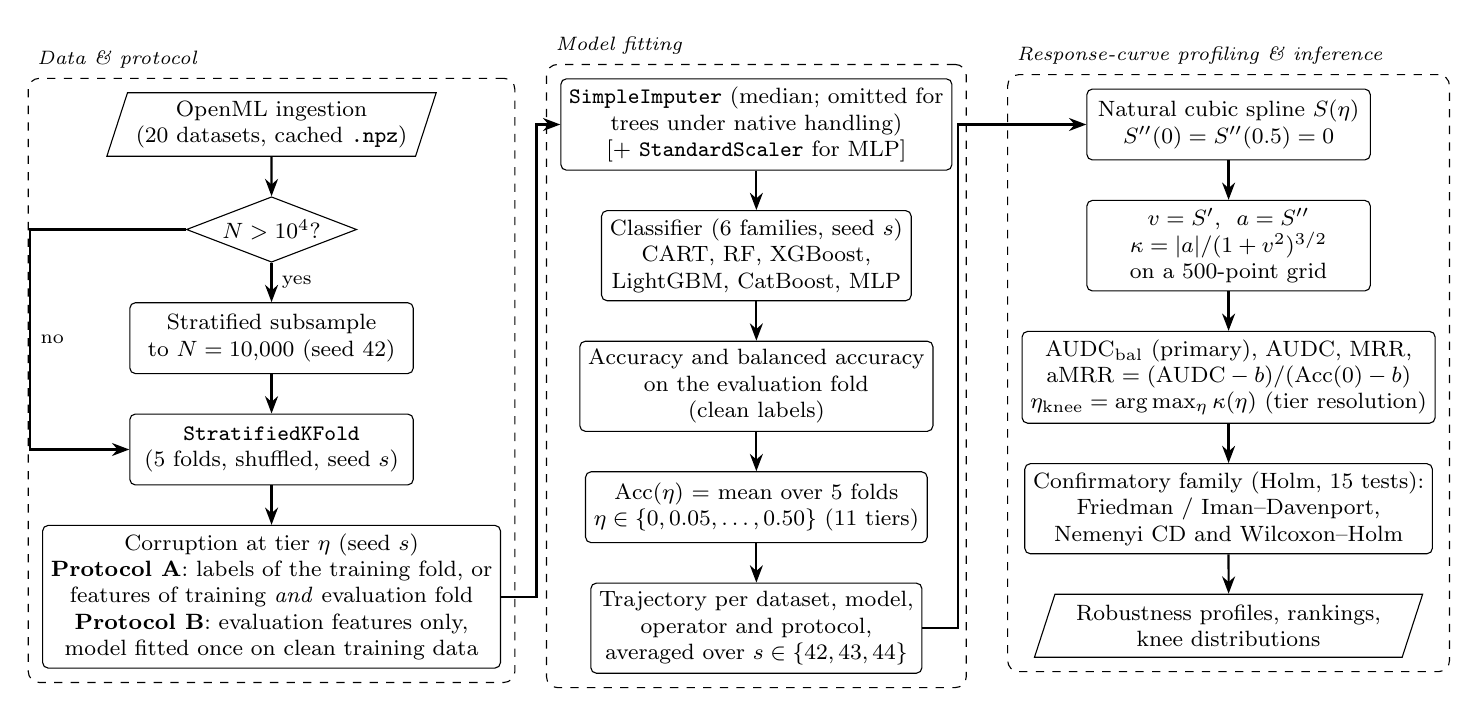
\begin{tikzpicture}[
  node distance=5mm and 7mm,
  every node/.style={font=\footnotesize, align=center},
  proc/.style={rectangle, draw, rounded corners=2pt, minimum width=36mm, minimum height=9mm, inner sep=3pt},
  data/.style={trapezium, trapezium left angle=72, trapezium right angle=108, draw, minimum width=30mm, minimum height=8mm, inner sep=3pt},
  dec/.style={diamond, draw, aspect=2.6, inner sep=1pt},
  stage/.style={draw, dashed, rounded corners=4pt, inner sep=5pt},
  lab/.style={font=\scriptsize\itshape, anchor=south west},
  arr/.style={-{Stealth[length=2.2mm]}, thick}
]
% --- Column 1: data and evaluation protocol
\node[data] (ingest) {OpenML ingestion\\(20 datasets, cached \texttt{.npz})};
\node[dec, below=of ingest] (size) {$N > 10^4$?};
\node[proc, below=of size] (sub) {Stratified subsample\\to $N = 10{,}000$ (seed 42)};
\node[proc, below=of sub] (kfold) {\texttt{StratifiedKFold}\\(5 folds, shuffled, seed $s$)};
\node[proc, below=of kfold] (msnie) {Corruption at tier $\eta$ (seed $s$)\\\textbf{Protocol A}: labels of the training fold, or\\features of training \emph{and} evaluation fold\\\textbf{Protocol B}: evaluation features only,\\model fitted once on clean training data};

% --- Column 2: model fitting
\node[proc, right=17mm of ingest] (imp) {\texttt{SimpleImputer} (median; omitted for\\trees under native handling)\\{}[+ \texttt{StandardScaler} for MLP]};
\node[proc, below=of imp] (clf) {Classifier (6 families, seed $s$)\\CART, RF, XGBoost,\\LightGBM, CatBoost, MLP};
\node[proc, below=of clf] (acc) {Accuracy and balanced accuracy\\on the evaluation fold\\(clean labels)};
\node[proc, below=of acc] (mean) {$\mathrm{Acc}(\eta)$ = mean over 5 folds\\$\eta \in \{0, 0.05, \ldots, 0.50\}$ (11 tiers)};
\node[proc, below=of mean] (store) {Trajectory per dataset, model,\\operator and protocol,\\averaged over $s\in\{42,43,44\}$};

% --- Column 3: knee geometry and inference
\node[proc, right=17mm of imp] (spline) {Natural cubic spline $S(\eta)$\\$S''(0) = S''(0.5) = 0$};
\node[proc, below=of spline] (deriv) {$v = S'$, \ $a = S''$\\$\kappa = \lvert a\rvert / (1 + v^2)^{3/2}$\\on a 500-point grid};
\node[proc, below=of deriv] (metrics) {AUDC$_{\mathrm{bal}}$ (primary), AUDC, MRR,\\aMRR $=(\mathrm{AUDC}-b)/(\mathrm{Acc}(0)-b)$\\$\eta_{\mathrm{knee}}=\arg\max_\eta\kappa(\eta)$ (tier resolution)};
\node[proc, below=of metrics] (stats) {Confirmatory family (Holm, 15 tests):\\Friedman / Iman--Davenport,\\Nemenyi CD and Wilcoxon--Holm};
\node[data, below=of stats] (out) {Robustness profiles, rankings,\\knee distributions};

% --- Flow
\draw[arr] (ingest) -- (size);
\draw[arr] (size) -- node[right, font=\scriptsize]{yes} (sub);
\draw[arr] (size.west) -- (size.west -| msnie.west) -- ++(-1.5mm,0) |- node[pos=0.25, right, font=\scriptsize]{no} (kfold.west);
\draw[arr] (sub) -- (kfold);
\draw[arr] (kfold) -- (msnie);
\draw[arr] (msnie.east) -- ++(4.5mm,0) |- (imp.west);
\draw[arr] (imp) -- (clf);
\draw[arr] (clf) -- (acc);
\draw[arr] (acc) -- (mean);
\draw[arr] (mean) -- (store);
\draw[arr] (store.east) -- ++(4.5mm,0) |- (spline.west);
\draw[arr] (spline) -- (deriv);
\draw[arr] (deriv) -- (metrics);
\draw[arr] (metrics) -- (stats);
\draw[arr] (stats) -- (out);

% --- Stage boxes
\node[stage, fit=(ingest)(size)(sub)(kfold)(msnie)] (s1) {};
\node[lab] at (s1.north west) {Data \& protocol};
\node[stage, fit=(imp)(clf)(acc)(mean)(store)] (s2) {};
\node[lab] at (s2.north west) {Model fitting};
\node[stage, fit=(spline)(deriv)(metrics)(stats)(out)] (s3) {};
\node[lab] at (s3.north west) {Response-curve profiling \& inference};
\end{tikzpicture}%
}
\caption{The TabStress framework. For every cell (dataset, model, operator, $\eta$, seed $s$) the fold split, the corruption and the model are seeded with $s\in\{42,43,44\}$; the 10{,}000-row subsample is drawn once, with seed 42. Under Protocol~A (corruption-aware training robustness) label operators corrupt only the training labels and feature operators corrupt the training and the evaluation features at the same intensity, and the model is refitted at every intensity. Under Protocol~B (deployment robustness) the model is fitted once per fold on clean data and scored on evaluation features corrupted at every intensity. Predictions are always scored against clean labels.}
\label{fig:pipeline}
\end{figure}
%% ---- end inlined sections/methodology_flowchart.tex ----

\subsection{Corruption engine}\label{sec:method:engine}

The corruption engine implements the operators of Definition~\ref{def:operators}. Its random generator is seeded per cell, and the corruption of a trajectory is coupled across tiers (with the exception noted below): under Protocol~A an entry masked or a label flipped at one intensity is masked or flipped in the same way at every higher intensity, and Gaussian perturbations grow in proportion to $\eta$, so adjacent tiers differ by the added corruption only. (The exception is symmetric noise on the six multiclass datasets, where replacement labels consume an $\eta$-dependent number of draws; there the corrupted examples are coupled in the first fold only, and their new labels in none.) Under Protocol~B each tier of each evaluation fold receives its own seeded draw. The engine was audited against Definition~\ref{def:operators} on all twenty datasets: realized label-flip rates lie within 2.0 binomial standard errors of $\eta$, every pair-flip moves a label to the successor class, minority-to-majority noise never alters the other class, the realized Gaussian variance of each non-constant column lies within 3.8 standard errors of $\eta^{2}\sigma_j^{2}$, and the realized MCAR rate within 1.9 standard errors of $\eta$. MAR and MNAR rates average $\eta$ by construction, with maximum per-entry probability $2\eta\le1$. The coupling of the tiers described above was confirmed fold by fold for every operator and dataset, and none of the 300 blocks of the Protocol~A grid (seed, condition and dataset) is constant across intensities for every model; a corruption operator that changed nothing would produce constant blocks, so this check rules out a no-op operator, apart from the three Gaussian blocks (one per seed) of amazon\_access, a dataset with no continuous attribute, on which the principal operator has nothing to perturb and which is flat by construction.

\subsection{Model configurations}\label{sec:method:models}

The six families span the inductive biases that dominate tabular practice: a CART tree~\cite{breiman1984classification}; a random forest (RF) of 100 trees~\cite{breiman2001random}; XGBoost~\cite{chen2016xgboost}, LightGBM~\cite{ke2017lightgbm} and CatBoost~\cite{prokhorenkova2018catboost}, each with 100 boosting rounds at learning rate $0.1$; and a multilayer perceptron (MLP) with hidden layers of 128, 64 and 32 units, at most 300 epochs and early stopping on a 10\% hold-out of the training fold. All other MLP settings are scikit-learn defaults (Adam, initial learning rate $10^{-3}$, L2 penalty $\alpha=10^{-4}$, batch size $\min(200,n)$, $10$ epochs without improvement, tolerance $10^{-4}$). The MLP is the classical dense baseline. Under Protocol~A its early-stopping hold-out is drawn from the corrupted training labels. An ablation with early stopping disabled under symmetric label noise was run across all twenty datasets (Section~\ref{sec:res:label}). Every pipeline begins with median imputation fitted on the training fold, and the MLP adds standardization. Under native handling the imputer is removed for the five tree families: the scikit-learn trees, XGBoost and LightGBM learn at each split which branch receives a missing value, and CatBoost treats missing values as smaller than every observed value. The MLP keeps its imputer in every condition.

Three configuration regimes separate \emph{model-family robustness}, the corruption response of a family under one fixed configuration, from \emph{configuration robustness}, how far that response changes when hyperparameters or training budget change within a family:
\begin{itemize}
\item \emph{Matched budget} (all seeds, all operators): the configuration above. It coincides with the library defaults of CART, RF and LightGBM.
\item \emph{Library defaults} (seed 42, four Protocol~A operators): XGBoost with learning rate $0.3$ and CatBoost with 1,000 rounds and an automatically chosen learning rate.
\item \emph{Tuned} (seed 42, on all twenty datasets): for each dataset and family, six configurations drawn at random from a fixed search space (Supplementary Table~S1) are compared by three-fold cross-validated accuracy (not the primary balanced score) on the clean training part of the first outer fold; the best configuration is then run under symmetric label noise and Gaussian noise (Protocol~A) and Gaussian noise (Protocol~B) on the same folds as the matched budget. With only six clean-data trials per family, this search shows configuration sensitivity; it does not establish ranking stability under comprehensive tuning or tuning for corruption robustness.
\end{itemize}
The six families are \emph{classical supervised tabular learners}, trained from scratch in every fold, and they carry every confirmatory claim of this study. A seventh, pretrained family is added as an exploratory, secondary, inference-time baseline in response to the question whether the findings extend to tabular foundation models~\cite{hollmann2023tabpfn}: TabICL~\cite{qu2025tabicl}, an open model that classifies by in-context learning, conditioning on the labeled training rows in a single forward pass without parameter updates. It is evaluated under Protocol~B only. Under Protocol~A it would have to be refitted at every intensity and fold, and for an in-context learner that means repeating inference over the whole corrupted training fold in every cell, which was beyond the compute budget. Under Protocol~B the clean training fold is its context, and it predicts each corrupted copy of the validation fold, on the same folds and with the same corruption draws as the six classical families. The run uses tabicl 2.2.0, whose default classifier checkpoint (\texttt{tabicl-classifier-v2-20260212}) is the TabICLv2 release~\cite{qu2025tabicl}, evaluated with PyTorch 2.14.1. Four constraints were imposed for computational tractability: (i) an ensemble of four members instead of the default eight, (ii) an in-context set limited to 3{,}000 rows (a stratified subsample of the training fold, seeded per seed and fold), (iii) median imputation fitted on the clean training fold before the model, so that TabICL never receives a missing value. and (iv) Bioresponse ($D=1{,}776$) was excluded to keep the inference setting uniform across the corpus: under the standardized budget (3{,}000 context rows, four estimators) its column-wise embedding exceeded the available memory, so the comparison covers nineteen of the twenty datasets. The exclusion is therefore a compute limitation of this study, not a property of the model. Because of these constraints the scores describe this specific configuration; we make no claim that they are a lower bound on what the model can attain, since the constraints could raise or lower any score. TabICL is a single model evaluated under constrained settings and one protocol; we avoid generalizing these results to foundation models as an entire class.

\subsection{Experimental protocol}\label{sec:method:protocol}

\paragraph{Dataset selection.} The corpus is fixed by explicit criteria, stated here so that it can be audited and extended: (i) a public classification task with a stable OpenML identifier~\cite{bischl2021openml}, in its original upload; (ii) membership of an established benchmarking suite (OpenML-CC18, the AutoML Benchmark, OpenML100) or use in published tabular comparisons; (iii) at least 800 rows, so that each of the five evaluation folds holds about 160 rows, with a cap of ten thousand rows to bound compute (the corpus ranges from 846 to 130{,}064 rows); (iv) both binary and multiclass tasks, here $K=2$ to $11$; (v) majority-class rates from balanced to severely imbalanced, here $\pi_{\max}=0.22$ to $0.94$; (vi) a spread of dimensionality, here $D=5$ to $1{,}776$ encoded columns, and of the share of integer-coded columns, from purely real-valued to purely discrete; (vii) application domains from science and sensing, industry, business and the web, and synthetic or perceptual tasks; and (viii) no missing values in the upload, so that every masking operator acts on fully observed matrices. Excluded were regression tasks, datasets requiring text, image or time-series processing, and tasks with fewer than about 800 rows. Twenty datasets give a Nemenyi critical difference of $\mathrm{CD}=1.686$ at $\alpha=0.05$; this is the resolution limit of the pairwise comparisons, and Section~\ref{sec:res:stats} shows that it separates only a minority of model pairs. The corpus spans diverse operational profiles, and the protocol requires over 111{,}000 model fits. Twenty curated public datasets still cannot represent uncurated industrial data, a boundary this study keeps in view throughout. Table~\ref{tab:inventory} lists the resulting twenty datasets; preprocessing details are in Supplementary Table~S2. Categorical attributes with at most 25 levels are dummy-coded and the others ordinally encoded. Nine datasets exceed $10{,}000$ rows and are reduced once to exactly $10{,}000$ rows by stratified sampling with seed 42, so that all models, operators, intensities and seeds see the same rows.

%% ---- begin inlined ../results/analysis/revision/tab_inventory_main.tex ----
\begin{table}[t]
\centering
\footnotesize
\caption{Benchmark corpus. $N$: rows (after the one-off stratified cap of 10{,}000); $D$: encoded columns; $K$: classes; $\pi_{\max}$: majority-class rate; type: share of integer-coded columns (real-valued when 0\%, discrete when 100\%). OpenML identifiers and preprocessing details are in Supplementary Table~S2.}
\label{tab:inventory}
\begin{tabular}{@{}llrrrrl@{}}
\toprule
Dataset & Domain & $N$ & $D$ & $K$ & $\pi_{\max}$ & Type \\
\midrule
Bioresponse & Science & 3{,}751 & 1{,}776 & 2 & 0.54 & mixed (47\%) \\
qsar-biodeg & Science & 1{,}055 & 41 & 2 & 0.66 & mixed (59\%) \\
eye\_movements & Science & 10{,}000 & 27 & 3 & 0.39 & mixed (67\%) \\
gesture\_phase & Science & 9{,}873 & 32 & 5 & 0.30 & real \\
ozone\_level & Science & 2{,}534 & 72 & 2 & 0.94 & real \\
steel-plates-fault & Industrial & 1{,}941 & 33 & 2 & 0.65 & mixed (61\%) \\
vehicle & Sensing (silhouettes) & 846 & 18 & 4 & 0.26 & discrete \\
electricity & Industrial & 10{,}000 & 13 & 2 & 0.58 & mixed (46\%) \\
pol & Industrial & 10{,}000 & 48 & 11 & 0.62 & discrete \\
miniboone & Physical sciences (neutrino detection) & 10{,}000 & 50 & 2 & 0.72 & real \\
bank-marketing & Business, web & 10{,}000 & 42 & 2 & 0.88 & discrete \\
churn & Business, web & 5{,}000 & 29 & 2 & 0.86 & mixed (72\%) \\
amazon\_access & Business, web & 10{,}000 & 9 & 2 & 0.94 & discrete \\
nomao & Business, web & 10{,}000 & 145 & 2 & 0.71 & mixed (39\%) \\
spambase & Business, web & 4{,}601 & 57 & 2 & 0.61 & mixed (4\%) \\
madelon & Synthetic, other & 2{,}600 & 500 & 2 & 0.50 & discrete \\
hill\_valley & Synthetic, other & 1{,}212 & 100 & 2 & 0.50 & real \\
jungle\_chess & Synthetic, other & 10{,}000 & 6 & 3 & 0.51 & discrete \\
phoneme & Synthetic, other & 5{,}404 & 5 & 2 & 0.71 & real \\
volkert & Synthetic, other & 10{,}000 & 180 & 10 & 0.22 & mixed (18\%) \\
\bottomrule
\end{tabular}
\end{table}
%% ---- end inlined ../results/analysis/revision/tab_inventory_main.tex ----

\paragraph{Duplicate rows and cleaning.} Three uploads contain artifacts that are handled in Section~\ref{sec:res:config}: duplicate feature rows in spambase (cleaned, with conflicting duplicates dropped), an identifier column in churn (dropped) and sentinel rows in MiniBooNE (removed). The spambase cleaning removes 391 duplicate rows (rule R1, first occurrence kept) and 6 rows forming 3 conflicting feature vectors (rule R2), 397 rows in all; MiniBooNE loses 468 rows whose features all equal $-999.0$. Five further datasets contain exact duplicate feature rows that the primary grid retains: nomao (2,405 of 34,465 rows in the full upload), pol (42), volkert (12), phoneme (9) and ozone\_level (8). The counts are reproduced by \texttt{experiments/duplicate\_scan.py}. Corrections and sensitivity runs are indexed with their scripts and summaries in PIPELINE\_MANIFEST.md (Section~5.4). The cleaned-copy sensitivity analysis for these five datasets is reported in the artifact-sensitivity subsection of the results: with them substituted, the best and the worst model are unchanged in all fifteen confirmatory blocks. We therefore report two versions of the corpus as a dual-protocol data-integrity audit: the standard OpenML distribution uploads (the primary grid) and a deduplicated corpus (all 4,440 cells, seeds 42--44; Table~\ref{tab:sensitivity}). Removing the duplicate rows leaves the best and worst model unchanged in all fifteen confirmatory blocks and keeps fourteen of fifteen omnibus tests significant after Holm adjustment. Intermediate ranks do move (minimum Kendall $\tau=0.83$), and no balanced-AUDC trajectory changes by more than $0.006$. Contamination therefore does not change which models lead or trail, but it does shift the middle of the ranking.

\paragraph{Benchmark overlap.} Sixteen datasets belong to OpenML-CC18 (thirteen; OpenML suite 99) or to the AutoML Benchmark (three more: miniboone, volkert and amazon\_access; suite 271), which we checked against the suite identifiers. Four datasets (eye\_movements, steel-plates-fault, pol and hill\_valley) belong to neither suite and were included because they appear in published tabular comparisons. Seven of the twenty datasets overlap with the numerical benchmark suite of Grinsztajn et al.~\cite{grinsztajn2022tree} (Bioresponse, electricity, eye\_movements, bank-marketing, phoneme, qsar-biodeg and madelon). The clean-accuracy component of our results is therefore an independent re-measurement on familiar data, not new evidence about clean performance; the robustness trajectories, by contrast, are new measurements. The six classical families are trained from scratch in every fold and have no pretraining exposure; TabICL is pretrained on synthetic priors~\cite{qu2025tabicl} that are not known to include these datasets, but exposure cannot be fully excluded, which is one reason its results are secondary. What the overlap does carry is the common risk of a community-wide focus on a few public datasets, which Section~\ref{sec:threats} discusses as benchmark selection bias.

\paragraph{Cells and fits.} Counts in this article rest on three terms. An \emph{evaluation cell} (or \emph{cell}) is a distinct combination of dataset, model family, corruption operator, intensity tier $\eta$, and random seed, evaluated by stratified five-fold cross-validation; a \emph{model fit} is a single model training event on one training fold; and an \emph{evaluation} is the scoring of one fitted model on one evaluation fold at one corruption tier. A cell therefore comprises five evaluations. Under Protocol~A each cell entails five model fits; under Protocol~B the five fits per dataset, model and seed are shared by all eleven tiers. The abstract, Table~\ref{tab:accounting} and the replication documentation use these three terms only in this sense. Table~\ref{tab:accounting} derives every count quoted in this article. The primary grid of the five original conditions (symmetric and class-conditional label noise, Gaussian noise, MCAR with imputed and with native handling) has $20\times6\times5\times11\times3=19{,}800$ rows, but its clean cells are shared by all five conditions and its native-handling MLP rows are the imputed ones; it rests on 17{,}760 distinct cells. Together with the pair-flip runs on the binary datasets that serve as a test--retest control (Section~\ref{sec:res:knee}), the duplicate clean cells of the original seed-42 run and the library-default runs, the Protocol~A grid comprises 22{,}280 cross-validated cells and 111{,}400 model fits.

\paragraph{Protocol~B accounting.} The 25{,}740 Protocol~B cells are the Gaussian rows (3{,}960) and the MCAR, MAR and MNAR rows (7{,}260 each). Each masking mechanism contributes 3{,}960 imputed rows and 3{,}300 native-tree rows. The 3{,}300 model fits are 1{,}800 for the six families under the imputed pipeline (20 datasets $\times$ 6 families $\times$ 3 seeds $\times$ 5 folds) and 1{,}500 for the five tree families under native handling (20 $\times$ 5 $\times$ 3 $\times$ 5). Native fits are shared across MCAR, MAR and MNAR, and the categorical and continuous-Gaussian Protocol~B cells reuse the clean-trained fits. TabICL (2{,}508 cells, 285 fits) and the tuned configurations are reported separately and are not included in these totals.

%% ---- begin inlined ../results/analysis/revision/tab_accounting.tex ----
\begin{table}[t]
\centering
\footnotesize
\caption{Derivation of the cell and fit counts. A cell is one dataset, model, operator, intensity and seed evaluated by five-fold cross-validation (five model fits under Protocol~A; under Protocol~B one fit per fold serves all tiers). An evaluation scores one fitted model on one evaluation fold at one tier, so a cell comprises five evaluations; the rows below count cells. The primary grid reuses each clean cell in all five conditions and the imputed MLP rows in the native condition.}
\label{tab:accounting}
\begin{tabular}{@{}p{3.3cm}p{5.2cm}r@{}}
\toprule
Block & Factors & Cells \\
\midrule
Original run, seed 42 & $20\times6\times4$ operators $\times\,11$ tiers & 5{,}280 \\
Seeds 43, 44 & $2\times20\times6\times(1\text{ clean}+4\times10)$ & 9{,}840 \\
Minority-to-majority & $3\times14$ binary datasets $\times\,6\times10$ & 2{,}520 \\
Native handling & $3\times20\times5$ tree families $\times\,10$ & 3{,}000 \\
Library defaults & $2$ libraries $\times\,20\times(1+4\times10)$, seed 42 & 1{,}640 \\
\midrule
Protocol A total & cells / model fits & 22{,}280 / 111{,}400 \\
\quad of which primary & $3\times(120\text{ clean}+5{,}800\text{ noisy})$ & 17{,}760 \\
\quad pair-flip on binary & test--retest control, $3\times14\times6\times10$ & 2{,}520 \\
\quad duplicate clean & seed-42 clean cells of three extra operators & 360 \\
\quad library defaults & $2\times20\times(1+4\times10)$, seed 42 & 1{,}640 \\
Primary grid rows & $20\times6\times5\times11\times3$ & 19{,}800 \\
Protocol B & cells / model fits & 25{,}740 / 3{,}300 \\
TabICL (B) & cells / model fits, seeds 42--44, 19 datasets & 2{,}508 / 285 \\
MAR, MNAR (A) & cells, seeds 42--44 & 7{,}200 \\
Tuned configurations & cells, seed 42 & 3{,}960 \\
Categorical (B) & cells, seeds 42--44 & 2{,}376 \\
Categorical (A) & cells, seeds 42--44 & 2{,}160 \\
\bottomrule
\end{tabular}
\end{table}
%% ---- end inlined ../results/analysis/revision/tab_accounting.tex ----

\begin{algorithm}[t]
\caption{Evaluation of one trajectory $(\mathcal{D},m,\omega,s)$ under Protocol~A or~B}\label{alg:cell}
\begin{algorithmic}[1]
\Require data $(\mathbf{X},\mathbf{y})$ with $N\le10^{4}$, model family $m$, operator $\omega$, seed $s$, protocol $P$
\State $\mathcal{F}\gets$ stratified 5-fold split (seed $s$)
\For{each fold $(\mathcal{I}_{\mathrm{tr}},\mathcal{I}_{\mathrm{va}})\in\mathcal{F}$}
  \If{$P=\mathrm{B}$} \State fit imputer, scaler and $m$ (seed $s$) once on the clean $(\mathbf{X}_{\mathrm{tr}},\mathbf{y}_{\mathrm{tr}})$ \EndIf
  \For{each tier $\eta\in\{0,0.05,\dots,0.5\}$}
    \If{$P=\mathrm{A}$ and $\omega$ is a label operator}
      \State $\tilde{\mathbf{y}}_{\mathrm{tr}}\gets\mathcal{T}_{\omega,\eta}(\mathbf{y}_{\mathrm{tr}})$; \quad $\tilde{\mathbf{X}}_{\mathrm{tr}}\gets\mathbf{X}_{\mathrm{tr}}$, \ $\tilde{\mathbf{X}}_{\mathrm{va}}\gets\mathbf{X}_{\mathrm{va}}$
    \ElsIf{$P=\mathrm{A}$}
      \State $\tilde{\mathbf{X}}_{\mathrm{tr}}\gets\mathcal{T}_{\omega,\eta}(\mathbf{X}_{\mathrm{tr}})$, \ $\tilde{\mathbf{X}}_{\mathrm{va}}\gets\mathcal{T}_{\omega,\eta}(\mathbf{X}_{\mathrm{va}})$; \quad $\tilde{\mathbf{y}}_{\mathrm{tr}}\gets\mathbf{y}_{\mathrm{tr}}$
    \Else
      \State $\tilde{\mathbf{X}}_{\mathrm{va}}\gets\mathcal{T}_{\omega,\eta}(\mathbf{X}_{\mathrm{va}})$ \Comment{training data stay clean}
    \EndIf
    \If{$P=\mathrm{A}$} \State fit imputer (unless native), scaler (MLP) and $m$ on $(\tilde{\mathbf{X}}_{\mathrm{tr}},\tilde{\mathbf{y}}_{\mathrm{tr}})$ \EndIf
    \State $a_{f,\eta},\ b_{f,\eta}\gets$ accuracy and balanced accuracy of $m(\tilde{\mathbf{X}}_{\mathrm{va}})$ against the clean $\mathbf{y}_{\mathrm{va}}$
  \EndFor
\EndFor
\State \Return $\bigl(\tfrac15\sum_f a_{f,\eta},\ \tfrac15\sum_f b_{f,\eta}\bigr)_{\eta}$
\end{algorithmic}
\end{algorithm}

\paragraph{Pipeline verification and numerical stability.} Evaluation pipelines were subjected to independent numerical verification: zero-variance safeguards ($\sigma_j=0$) prevent artificial perturbation on constant columns, and minority-class selection under balanced binary targets is deterministically resolved. These corrections were identified during independent pipeline validation and were applied before the final statistical analysis. Recomputing the seed-42 Gaussian ranking with the values before the constant-column correction leaves LightGBM first and CART last; the largest mean-rank change is 0.40 (MLP) and the largest single-trajectory change in balanced AUDC is 0.20. The values before the minority-class correction were not retained, so its effect is not quantified. Every number in this article is computed by one final run of the analysis on the corrected cell files%
, and a random sample of 120 stored cells, drawn from every block and seed, was recomputed from scratch with the corrected harness and agrees with the stored values to within $1.1\times10^{-16}$%
. The replication package includes complete pipeline scripts, output files, and verification checks. Stored evaluations replicate deterministically across independent execution environments.

\paragraph{Implementation.} The harness is implemented in Python 3.12.6 with scikit-learn 1.9.1, XGBoost 3.4.1, LightGBM 4.7.0, CatBoost 1.2.10 and autorank 1.3.0; the MLP is scikit-learn's \texttt{MLPClassifier}. Classical models run on multi-core CPU workers; TabICL runs in an isolated virtual environment with tabicl 2.2.0 and PyTorch 2.14.1.

\paragraph{Use of AI tools.} During the preparation of this manuscript, automated language assistance tools were utilized exclusively for grammar verification, stylistic consistency, and language copyediting. The authors designed the study, conducted all empirical benchmarking and theoretical analyses, verified all outputs against stored data, and take full responsibility for the content.

\subsection{Statistical analysis}\label{sec:method:stats}

The unit of inference is the dataset. For each condition and score, the six models are ranked within each dataset (rank 1 for the highest score, ties averaged) and $R_j$ is the mean rank of model $j$ over $N=20$ datasets. With $k=6$, the Friedman statistic and its Iman--Davenport correction are given in Equation~\eqref{eq:friedman}
\begin{equation}\label{eq:friedman}
\chi^{2}_{F}=\frac{12N}{k(k+1)}\Bigl[\sum_{j=1}^{k}R_j^{2}-\frac{k(k+1)^{2}}{4}\Bigr],\qquad
F_F=\frac{(N-1)\chi^{2}_{F}}{N(k-1)-\chi^{2}_{F}}\sim F(5,95).
\end{equation}
Two models differ under the Nemenyi procedure if their mean ranks differ by more than $\mathrm{CD}=q_{0.05}\sqrt{k(k+1)/(6N)}=1.686$, with $q_{0.05}=2.850$ for $k=6$ and $N=20$. Because a mean-rank verdict depends on the pool~\cite{benavoli2016should}, all fifteen pairwise Wilcoxon signed-rank tests are also run, with Holm adjustment over the fifteen pairs. Shapiro--Wilk rejects normality of the per-dataset scores for up to two of the six models within a condition. With $N=20$ this test has low power, so the rejection is treated as a warning, not a proof; the Friedman-based analysis is non-parametric by construction and does not depend on normality. \texttt{autorank}~\cite{herbold2020autorank} is run on its non-parametric route for the same reason.

\paragraph{Hypothesis testing framework and family-wise error control.} To control Type~I error across multiple comparisons without inflating false discovery rates, statistical evaluations are partitioned into a primary confirmatory family of fifteen tests alongside a broader thirty-test comprehensive suite with Holm step-down error control. The confirmatory family was fixed after the initial benchmark runs had been completed. It consists of the Iman--Davenport tests of the primary measure, balanced AUDC, and of the two confirmatory measures, AUDC and MRR, under the five primary conditions: fifteen tests, with Holm's step-down procedure applied jointly over all fifteen, so that no metric has a separate error budget. To evaluate ranking stability across the full parameter space, we also report the broader thirty-test family, where 26 of 30 tests reject equal ranks. The sensitivity measures ($\MRR_{\mathrm{bal}}$, aMRR, $\aMRR_{\mathrm{bal}}$) are reported with Holm adjustment over the full set of thirty tests and are not used to support a claim on their own. Protocol~B, the additional missingness mechanisms, the categorical operators and the configuration experiments are secondary analyses, each with Holm adjustment within its block. $\etaknee$ is descriptive and is not tested.

%% ===========================================================================
\section{Experimental Results}\label{sec:results}

\subsection{Overall robustness performance}\label{sec:res:overall}

Figure~\ref{fig:curves} shows representative trajectories and Figure~\ref{fig:overall} the distribution of the primary measure over the twenty datasets for every model, condition and protocol; the per-dataset trajectories of all conditions are in the degradation atlas of Supplementary Section~S7.

\begin{figure}[t]
\centering
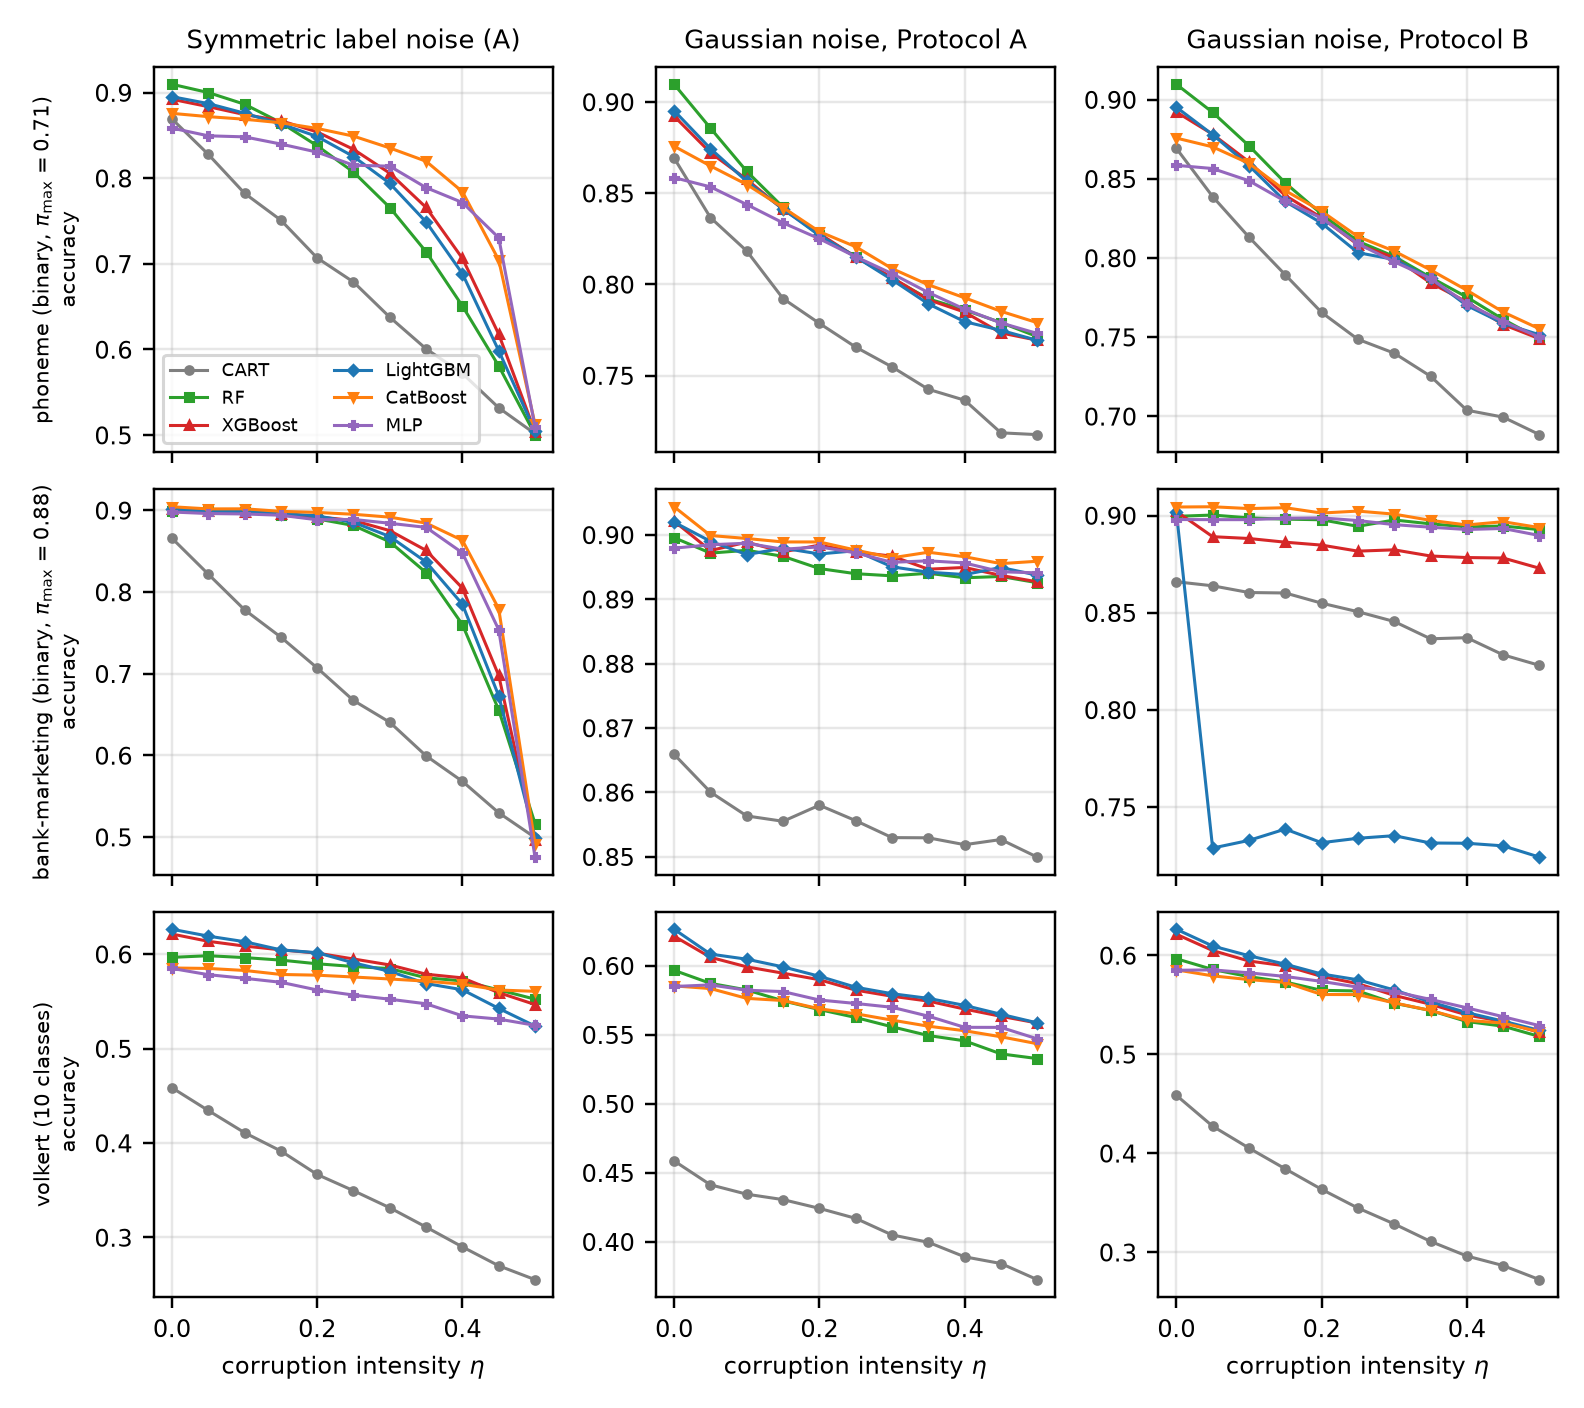
\includegraphics[width=0.75\linewidth]{fig_curves.png}
\caption{Representative degradation curves (plain accuracy averaged over seeds 42--44; the primary measure, balanced AUDC, is shown in Figure~\ref{fig:overall}): phoneme (binary, majority-class rate 0.71), bank-marketing (binary, majority-class rate 0.88) and volkert (ten classes), under symmetric label noise and under Gaussian feature noise, for training robustness (Protocol~A, corrupted training and test data) and inference robustness (Protocol~B, clean training, corrupted test data).}
\label{fig:curves}
\end{figure}

\begin{figure}[t]
\centering
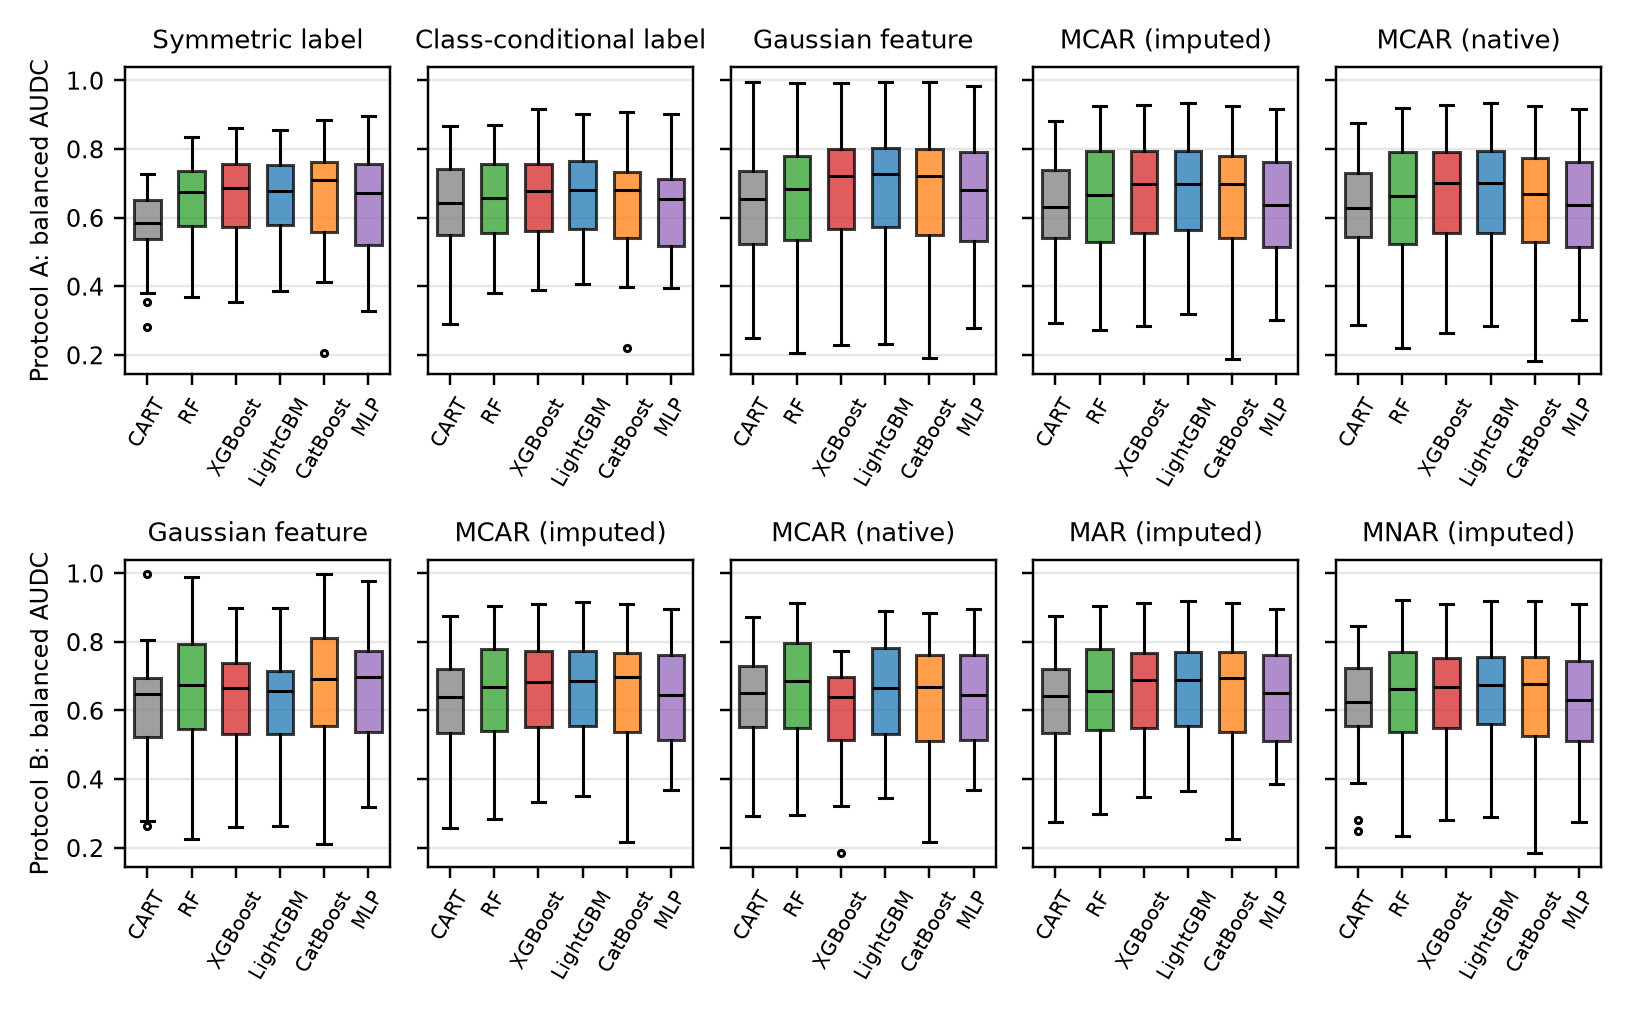
\includegraphics[width=0.75\linewidth]{fig_overall.png}
\caption{Balanced AUDC, the primary robustness measure, of every model over the twenty datasets. Top: training robustness (Protocol~A) under the five primary conditions. Bottom: inference robustness (Protocol~B) under Gaussian noise and under MCAR (imputed and native handling), MAR and MNAR masking (imputed). Boxes span the interquartile range; whiskers extend to $1.5$ times the interquartile range.}
\label{fig:overall}
\end{figure}

On the primary measure the six families differ under every condition (Table~\ref{tab:combined}; largest Holm-adjusted $p=2.1\times10^{-6}$). Three questions are kept apart throughout: whether the mean ranks differ across datasets (omnibus test), which model pairs are separated (pairwise tests), and whether the difference is practically meaningful (Kendall's $W$ and score differences). Under the matched 100-round budget, LightGBM has the best mean rank on balanced AUDC under four of the five conditions and CatBoost under symmetric label noise. When CatBoost runs at its library default of 1{,}000 rounds, it overtakes LightGBM under Gaussian noise (Section~\ref{sec:res:config}). At the bottom of the ranking, CART is last under four conditions and the MLP under class-conditional noise. For the five balanced-AUDC blocks in that sentence (symmetric, class-conditional, Gaussian, MCAR imputed, MCAR native), the Holm-adjusted Wilcoxon and Nemenyi tests separate 5/4, 8/5, 6/5, 8/6 and 9/7 of the fifteen model pairs; the omnibus rejection is not evidence of a complete ordering. Under class-conditional, Gaussian and both MCAR handlings, the Bayesian signed-rank test puts 0.80--0.90 of the posterior mass of LightGBM versus XGBoost inside the practical-equivalence region (ROPE $\pm0.01$ on balanced AUDC; Supplementary Table~S54), and the posterior probability that LightGBM wins is 0.00 in three of these conditions and 0.01 under imputed MCAR. These two families form a statistically equivalent top-performing tier in those conditions; we do not claim that LightGBM dominates XGBoost. Under symmetric label noise the best two families, CatBoost and XGBoost, have a ROPE probability of 0.36, and that condition does not show an equivalent top tier.

The answer to RQ1 is negative. Within a dataset and condition, the model with the highest clean accuracy also has the highest balanced AUDC in only 46\% of the hundred dataset--condition blocks, and the highest MRR in 4\%. The second figure reflects the denominator of MRR (Section~\ref{sec:problem:metrics}). We therefore treat the balanced-AUDC figure as the substantive answer to RQ1 and the MRR figure as a description of what relative retention measures. The median within-dataset Kendall correlation between clean accuracy and MRR is negative under every condition (from $-0.27$ to $-0.13$): the models that are most accurate on clean data tend to lose the largest share of it. Absolute endurance inherits part of the clean ordering, because a model that starts higher has more to spend, but clean accuracy alone does not identify the most robust model.

%% ---- begin inlined ../results/analysis/revision/tab_combined.tex ----
\begin{table*}[t]
\centering
\footnotesize
\caption{Cross-model comparison on the primary grid (Protocol~A, $N=20$ datasets, $k=6$ models, seed-averaged). Best and worst: lowest and highest mean Friedman rank (in parentheses). $p$: Iman--Davenport $p$-value (omnibus: do mean ranks differ?), Holm-adjusted over the confirmatory family of 15 tests (upper block) or over the sensitivity family, i.e.\ jointly over all 30 tests (lower block). $W$: Kendall's coefficient of concordance, the effect size of the Friedman test (0: no agreement among datasets, 1: identical ranking on every dataset). Pairs: model pairs separated by Holm-adjusted Wilcoxon / Nemenyi (CD$=1.686$) out of 15 (pairwise support). $W$ is the practical magnitude of the ordering; a small $p$ with low $W$ and few separated pairs is not a stable ordering. Metric interpretations: $\AUDC_{\mathrm{bal}}$ (primary) measures absolute endurance under class imbalance; $\AUDC$ measures raw area under the degradation curve; $\MRR$ measures relative accuracy retention normalized by clean performance ($A_0$); $\MRR_{\mathrm{bal}}$, $\aMRR$ and $\aMRR_{\mathrm{bal}}$ are complementary views, not primary outcomes. The MLP is trained with early stopping on a hold-out of its training fold; the unablated comparison is in Section~\ref{sec:res:label}.}
\label{tab:combined}
\setlength{\tabcolsep}{4pt}
\begin{tabular}{@{}llllrrr@{}}
\toprule
Metric & Corruption & Best (rank) & Worst (rank) & adj.\ $p$ & $W$ & Sep.\ pairs (W/N) \\
\midrule
AUDC$_{\mathrm{bal}}$ & Symmetric & CatBoost (2.60) & CART (5.50) & $1.6\times10^{-8}$ & 0.39 & 5/4 \\
 & Class-cond. & LightGBM (2.15) & MLP (4.65) & $1.5\times10^{-6}$ & 0.32 & 8/5 \\
 & Gaussian & LightGBM (1.95) & CART (4.85) & $2.1\times10^{-6}$ & 0.31 & 6/5 \\
 & MCAR imp. & LightGBM (1.60) & CART (5.00) & $6.1\times10^{-11}$ & 0.47 & 8/6 \\
 & MCAR nat. & LightGBM (1.50) & CART (4.90) & $3.7\times10^{-12}$ & 0.50 & 9/7 \\
AUDC & Symmetric & CatBoost (2.15) & CART (5.85) & $2.8\times10^{-10}$ & 0.45 & 5/5 \\
 & Class-cond. & XGBoost (2.20) & CART (5.55) & $6.0\times10^{-13}$ & 0.52 & 8/6 \\
 & Gaussian & LightGBM (1.90) & CART (5.65) & $1.2\times10^{-12}$ & 0.52 & 9/6 \\
 & MCAR imp. & LightGBM (1.75) & CART (5.95) & $4.0\times10^{-21}$ & 0.68 & 13/7 \\
 & MCAR nat. & LightGBM (1.30) & CART (5.90) & $1.4\times10^{-26}$ & 0.76 & 14/8 \\
MRR & Symmetric & CatBoost (1.50) & CART (5.75) & $4.4\times10^{-21}$ & 0.68 & 12/8 \\
 & Class-cond. & MLP (2.60) & RF (4.45) & 0.026 & 0.12 & 1/1 \\
 & Gaussian & MLP (2.23) & CART (5.62) & $2.6\times10^{-10}$ & 0.45 & 9/6 \\
 & MCAR imp. & CatBoost (2.55) & CART (5.85) & $4.8\times10^{-9}$ & 0.41 & 5/5 \\
 & MCAR nat. & XGBoost (2.60) & CART (5.80) & $4.8\times10^{-9}$ & 0.41 & 5/5 \\
\midrule
\multicolumn{7}{@{}l}{\emph{Sensitivity metrics (not confirmatory)}}\\
MRR$_{\mathrm{bal}}$ & Symmetric & CatBoost (1.80) & CART (5.65) & $5.0\times10^{-11}$ & 0.48 & 8/5 \\
 & Class-cond. & XGBoost (3.15) & RF (3.85) & 0.879 & 0.02 & 0/0 \\
 & Gaussian & MLP (2.23) & CART (4.67) & $5.5\times10^{-5}$ & 0.28 & 4/5 \\
 & MCAR imp. & CatBoost (2.80) & CART (4.75) & 0.088 & 0.13 & 1/1 \\
 & MCAR nat. & XGBoost (2.70) & CART (4.65) & 0.023 & 0.16 & 0/2 \\
aMRR & Symmetric & CatBoost (1.60) & CART (5.40) & $2.7\times10^{-11}$ & 0.49 & 10/6 \\
 & Class-cond. & XGBoost (2.45) & CART (4.50) & 0.012 & 0.18 & 0/2 \\
 & Gaussian & CatBoost (2.40) & CART (5.45) & $1.4\times10^{-7}$ & 0.38 & 8/4 \\
 & MCAR imp. & CatBoost (2.55) & CART (5.75) & $1.4\times10^{-7}$ & 0.38 & 5/5 \\
 & MCAR nat. & XGBoost (2.20) & CART (5.70) & $1.1\times10^{-9}$ & 0.44 & 8/5 \\
aMRR$_{\mathrm{bal}}$ & Symmetric & CatBoost (2.08) & CART (5.65) & $2.7\times10^{-9}$ & 0.43 & 5/5 \\
 & Class-cond. & XGBoost (2.60) & MLP (4.22) & 0.088 & 0.11 & 1/0 \\
 & Gaussian & MLP (2.42) & CART (4.78) & 0.002 & 0.22 & 0/4 \\
 & MCAR imp. & LightGBM (2.65) & CART (4.85) & 0.011 & 0.18 & 0/2 \\
 & MCAR nat. & XGBoost (2.25) & CART (4.65) & $3.4\times10^{-5}$ & 0.29 & 4/4 \\
\bottomrule
\end{tabular}
\end{table*}
%% ---- end inlined ../results/analysis/revision/tab_combined.tex ----

\subsection{Label-noise robustness}\label{sec:res:label}

\paragraph{Symmetric noise.} CatBoost leads on all three confirmatory scores (Table~\ref{tab:combined}) and CART is last. LightGBM, the family with the highest mean clean accuracy over the twenty datasets (0.846), ranks fifth on MRR (mean rank 4.50 of six): its lead is spent early in the sweep. By Proposition~\ref{prop:a_symmetric}, what separates the models here is sample efficiency under an attenuated signal. The MLP, second on MRR, draws its early-stopping hold-out from the corrupted labels, an implicit form of noise-aware regularization that no other family receives; part of its relative retention may come from this rather than from the architecture. To test this confound we re-ran the MLP with early stopping disabled under symmetric label noise (seed 42, all twenty datasets, the same folds and corruption draws; \texttt{experiments/run\_mlp\_ablation.py}). Averaged over the ten noisy tiers, disabling early stopping lowers the MLP's balanced accuracy on fifteen of the twenty datasets (median difference $-0.025$; paired Wilcoxon $p=0.036$, $n=20$), and raises it on five. Early stopping on corrupted hold-out labels therefore helps the MLP on most datasets rather than inflating it. The effect is large on some datasets (nomao $-0.137$, pol $+0.111$), so the MLP's position under label noise depends on the training protocol. Recomputing the seed-42 symmetric-noise ranks with the ablated MLP in place of the primary one leaves the best and worst family unchanged on all three confirmatory scores, but moves the MLP from second to fifth on MRR and from third to fifth on AUDC (fifth on balanced AUDC in both cases). The MLP's retention advantage under symmetric label noise therefore depends on early stopping, and the ablation covers one seed.

\paragraph{Class-conditional noise.} Here Proposition~\ref{prop:a_minority} predicts that every learner follows the moved decision rule, and the families separate least: (i) Omnibus: MRR still differs after joint Holm adjustment ($p=0.026$). (ii) Pairwise: only one of the fifteen pairs is separated by the Wilcoxon tests. (iii) Magnitude: the agreement among datasets is weak ($W=0.12$), so the significant omnibus result does not indicate a stable or meaningful ordering. Balanced MRR does not distinguish the families at all (adjusted $p=0.879$). The variance of MRR between datasets is 15.4 times the variance between models, against 0.4 times under symmetric noise: how much accuracy is lost depends on the dataset far more than on the model. That bias shows in the gap between accuracy and balanced accuracy at the last tier: on the binary datasets the median terminal accuracy is 0.764 but the median terminal balanced accuracy only 0.585, whereas under symmetric noise the two coincide (0.499 and 0.499). On the four datasets with $\pi_{\max}\ge0.85$ terminal accuracy lies within 0.027 of the majority-class rate for every model. Much of the accuracy that survives class-conditional noise is earned by predicting the majority class, which is why the primary measure is balanced.

\subsection{Feature-noise and missingness robustness}\label{sec:res:feature}

Under corruption-aware training (Protocol~A), LightGBM leads on balanced AUDC and on AUDC under Gaussian noise and under both masking conditions, and CART is last (Table~\ref{tab:combined}). The MLP keeps a large share of its accuracy under Gaussian noise but ranks fifth on AUDC under imputed masking (mean rank 4.70 of six), where the median fill destroys the dependence between features on which it relies (Supplementary Proposition~S4).

\paragraph{Native versus imputed handling.} When missing values are present in training and evaluation data alike, native handling by the tree libraries changes the median AUDC of a family by at most $0.0030$ and never significantly improves on median imputation (Supplementary Table~S6); CART and CatBoost show small significant deficits (smallest Holm-adjusted $p=0.036$).

\paragraph{MAR and MNAR masking.} The additional operators were run under corruption-aware training on all twenty datasets, with seeds 42, 43 and 44 (scores are averaged over seeds when there are several). Table~\ref{tab:protocol}, lower block, compares them with Protocol~B on the same datasets and seeds. Under Protocol~A the families still differ on balanced AUDC under MAR and MNAR masking (largest Holm-adjusted $p=2.0\times10^{-11}$), with LightGBM leading under both. The remaining ranks are in Table~\ref{tab:protocol} and the supplement. At the same mean rate, self-masking MNAR costs more than MCAR: the median balanced AUDC under Protocol~A is 0.656 for MNAR and 0.675 for MCAR (twenty datasets, seed-averaged), whereas MAR gives 0.679, so the excess cost is not shown for MAR. A plausible reason for the MNAR result, which we have not tested, is that MNAR removes precisely the large values of every column and median imputation then fills them with a typical one.

\paragraph{Principal Gaussian experiment.} The Gaussian condition of this article perturbs continuous attributes only; Table~\ref{tab:gaussian_principal} sets it beside the all-column variant, which also perturbs label-encoded nominal codes and is retained as a mathematical stress test. The families differ on balanced AUDC under both protocols (Protocol~A $p=1.1\times10^{-6}$, Protocol~B $p=2.2\times10^{-4}$), with LightGBM best and CART worst under Protocol~A, and the mean-rank vectors agree closely with those of the all-column variant (Kendall $\tau=0.87$ under Protocol~A and $\tau=0.97$ under Protocol~B). On the six datasets with nominal attributes the continuous-only noise is the gentler one (median balanced AUDC higher by $+0.0041$ under Protocol~A, Wilcoxon $p=1.8\times10^{-7}$). One of the twenty datasets, amazon\_access, has no continuous attribute, so the principal operator leaves it untouched and its block is flat by construction; it is nevertheless kept in the confirmatory family, and Table~\ref{tab:amazon} reports the family with and without it. Omitting it leaves all fifteen tests significant after Holm adjustment and changes the best or worst model in one block (balanced AUDC under class-conditional noise: the worst model changes from the MLP to CART). The Gaussian results reported elsewhere are therefore not an artifact of perturbing encoded nominal codes.

\begin{table}[t]
\centering
\footnotesize
\caption{Confirmatory family with and without amazon\_access (fifteen tests, Holm-adjusted over the family as in Table~\ref{tab:combined}). Each cell gives the best and worst model by mean rank and the Iman--Davenport $p$-value. $\dagger$: the best or worst model changes when amazon\_access is removed. The principal Gaussian condition leaves amazon\_access untouched by construction.}
\label{tab:amazon}
\begin{tabular}{@{}llllll@{}}
\toprule
Score & Condition & \multicolumn{2}{c}{20 datasets} & \multicolumn{2}{c}{19 datasets (no amazon\_access)} \\
\cmidrule(lr){3-4}\cmidrule(lr){5-6}
 & & Best / worst & $p$ & Best / worst & $p$ \\
\midrule
AUDC$_{\mathrm{bal}}$ & Symmetric label & catboost / cart & $3.9\times10^{-9}$ & catboost / cart & $1.6\times10^{-10}$ \\
AUDC$_{\mathrm{bal}}$ & Class-conditional & lightgbm / mlp & $5.1\times10^{-7}$ & lightgbm / cart & $1.2\times10^{-7}$ $\dagger$ \\
AUDC$_{\mathrm{bal}}$ & Gaussian (principal) & lightgbm / cart & $1.1\times10^{-6}$ & lightgbm / cart & $7.5\times10^{-8}$ \\
AUDC$_{\mathrm{bal}}$ & MCAR, imputed & lightgbm / cart & $6.8\times10^{-12}$ & lightgbm / cart & $2.9\times10^{-13}$ \\
AUDC$_{\mathrm{bal}}$ & MCAR, native & lightgbm / cart & $3.7\times10^{-13}$ & lightgbm / cart & $6.3\times10^{-15}$ \\
AUDC & Symmetric label & catboost / cart & $4.0\times10^{-11}$ & catboost / cart & $2.5\times10^{-10}$ \\
AUDC & Class-conditional & xgboost / cart & $5.0\times10^{-14}$ & xgboost / cart & $1.2\times10^{-13}$ \\
AUDC & Gaussian (principal) & lightgbm / cart & $1.1\times10^{-13}$ & lightgbm / cart & $4.8\times10^{-13}$ \\
AUDC & MCAR, imputed & lightgbm / cart & $2.9\times10^{-22}$ & lightgbm / cart & $3.2\times10^{-21}$ \\
AUDC & MCAR, native & lightgbm / cart & $9.2\times10^{-28}$ & lightgbm / cart & $1.4\times10^{-27}$ \\
MRR & Symmetric label & catboost / cart & $3.4\times10^{-22}$ & catboost / cart & $1.1\times10^{-20}$ \\
MRR & Class-conditional & mlp / randomforest & 0.026 & mlp / randomforest & 0.041 \\
MRR & Gaussian (principal) & mlp / cart & $3.3\times10^{-11}$ & mlp / cart & $2.4\times10^{-12}$ \\
MRR & MCAR, imputed & catboost / cart & $9.2\times10^{-10}$ & catboost / cart & $6.3\times10^{-9}$ \\
MRR & MCAR, native & xgboost / cart & $8.0\times10^{-10}$ & xgboost / cart & $3.8\times10^{-9}$ \\
\bottomrule
\end{tabular}
\end{table}


%% ---- begin inlined ../results/analysis/revision/tab_gaussian_principal.tex ----
\begin{table}[t]
\centering
\footnotesize
\caption{The principal Gaussian condition against its all-column variant, 20 datasets, seeds 42--44. Principal: Gaussian noise on the continuous attributes only (nominal attributes left clean on the six datasets that have them; identical to the all-column operator on the other fourteen), the condition used throughout the article. All-column: the same noise on every encoded column, including label-encoded nominal codes; a mathematical stress test of representation resilience, not a realistic categorical error process. Omnibus $p$-values are unadjusted; the principal Gaussian condition belongs to the confirmatory family (Table~\ref{tab:combined}), where the corresponding tests are Holm-adjusted. $\tau$ compares the mean-rank vectors of the two variants.}
\label{tab:gaussian_principal}
\resizebox{\linewidth}{!}{%
\begin{tabular}{@{}llrrllrrrl@{}}
\toprule
Protocol & Variant & AUDC$_{\mathrm{bal}}$ $F$ & $p$ & Best & Worst & MRR $F$ & $p$ & Kendall $\tau$ & Same best/worst \\
\midrule
A (training) & Principal & 8.52 & $1.1\times10^{-6}$ & LightGBM & CART & 15.65 & $3.3\times10^{-11}$ & 0.87 & yes / yes \\
 & All-column & 8.73 & $7.7\times10^{-7}$ & LightGBM & CART & 19.60 & $2.3\times10^{-13}$ & -- & -- \\
B (inference) & Principal & 5.35 & $2.2\times10^{-4}$ & MLP & CART & 20.01 & $1.4\times10^{-13}$ & 0.97 & yes / yes \\
 & All-column & 4.84 & $5.5\times10^{-4}$ & MLP & CART & 22.95 & $4.9\times10^{-15}$ & -- & -- \\
\bottomrule
\end{tabular}%
}
\end{table}
%% ---- end inlined ../results/analysis/revision/tab_gaussian_principal.tex ----

\paragraph{Categorical corruption (separate analyses).} Table~\ref{tab:categorical} reports the two categorical operators on the six datasets with nominal attributes, under both protocols and three seeds. Replacing nominal values by valid but wrong categories costs slightly more than Gaussian noise on their codes: under corruption-aware training the median balanced AUDC of the categorical-aware operator is $-0.0063$ below that of the all-column Gaussian variant on the same folds (Wilcoxon $p=4.7\times10^{-4}$; the all-column variant is not the matched baseline for an operator that resamples rather than perturbs nominal codes), and under deployment the difference against the all-column variant is not significant ($p=0.114$). Against the matched principal Gaussian operator (continuous attributes only, same folds and seeds, 108 dataset--model--seed triples), the categorical-aware operator costs $-0.013$ balanced AUDC under Protocol~A and $-0.012$ under Protocol~B (Wilcoxon $p\approx10^{-18}$ in both); the categorical-only operator changes the median by $0.000$ under Protocol~A and $0.000$ under Protocol~B (Wilcoxon $p=0.063$ and $p=0.002$). The matched comparison is therefore the one to read, and the deployment effect against it is significant. Corrupting the nominal attributes alone costs little: the median loss of accuracy between $\eta=0$ and $\eta=0.5$ is 0.010 under Protocol~A and 0.015 under Protocol~B, so on these datasets most of the deterioration under feature noise comes from the continuous attributes. LightGBM has the highest mean balanced AUDC under every categorical condition. With six datasets these comparisons are descriptive; no rank test is reported.

%% ---- begin inlined ../results/analysis/revision/tab_categorical.tex ----
\begin{table}[t]
\centering
\footnotesize
\caption{Categorical corruption on the 6 datasets with nominal attributes (seeds 42--44). Categorical-aware: Gaussian noise on continuous attributes and whole-attribute resampling of nominal attributes; categorical-only: nominal attributes resampled, continuous attributes clean. $\Delta$: median over dataset--model pairs of balanced AUDC minus that of the all-column Gaussian operator on the same folds (the matched comparison with the principal operator is given in the text); $p$: Wilcoxon signed-rank test.}
\label{tab:categorical}
\begin{tabular}{@{}llrrrll@{}}
\toprule
Protocol & Operator & AUDC$_{\mathrm{bal}}$ & $\Delta$ vs.\ Gaussian & $p$ & Best & Worst \\
\midrule
A & categorical-aware & 0.657 & $-0.0063$ & $4.7\times10^{-4}$ & LightGBM & CART \\
 & categorical-only & 0.729 & $+0.0161$ & 0.004 & LightGBM & MLP \\
B & categorical-aware & 0.668 & $-0.0024$ & 0.114 & LightGBM & CART \\
 & categorical-only & 0.738 & $+0.0221$ & $3.1\times10^{-4}$ & LightGBM & MLP \\
\bottomrule
\end{tabular}
\end{table}
%% ---- end inlined ../results/analysis/revision/tab_categorical.tex ----


\subsection{Absolute versus relative endurance}\label{sec:res:absrel}

Absolute and relative scores answer different questions and rank the families differently. Under Gaussian noise and imputed masking LightGBM leads on AUDC (mean ranks 1.90 and 1.75), while the MLP leads on MRR under Gaussian noise and CatBoost under imputed masking; the MLP keeps a high share of an accuracy that was lower to begin with (mean AUDC 0.777 against 0.797 for LightGBM). Over the twenty-five comparisons of the primary measure with the five other scores, the Kendall correlation of the mean-rank vectors has median $0.47$ and minimum $-0.33$.

The baseline-adjusted ratio aMRR (Section~\ref{sec:problem:metrics}) is the check on relative leads. When the clean score exceeds the baseline by less than one point ($A_0-b<0.01$; Section~\ref{sec:problem:metrics}), above-baseline skill is negligible and $\aMRR$ is set to zero; in such uninformative regimes relative retention vanishes and absolute endurance ($\AUDC_{\mathrm{bal}}$) remains the sole reliable indicator. Under symmetric noise aMRR ranks the families exactly as MRR does and under Gaussian noise almost so (Kendall $\tau=0.97$), CatBoost is first on aMRR and the MLP on balanced aMRR (Table~\ref{tab:combined}), so the MLP's Gaussian retention lead does not survive the baseline adjustment on the unbalanced score. Under class-conditional noise the two disagree ($\tau=0.20$): the MLP's MRR lead disappears once the majority-class baseline is subtracted. Balanced AUDC is the primary measure; MRR and aMRR are complementary views and should be read together with it. Removing the zeroing rule (65 accuracy and 10 balanced trajectories) leaves the best and worst model unchanged in all but one aMRR block (the worst model under class-conditional noise changes from CART to random forest); for balanced aMRR under class-conditional noise the omnibus p rises from 0.043 to 0.22, so that sensitivity conclusion depends on the rule.

\subsection{Cross-model statistical comparison}\label{sec:res:stats}

All 15 tests of the confirmatory family reject the hypothesis of equal mean ranks after joint Holm adjustment (largest adjusted $p=0.026$, for MRR under class-conditional noise), with Kendall's coefficient of concordance between $W=0.12$ and $0.76$, from weak agreement among datasets about the order of the families (MRR under class-conditional noise) to strong agreement (AUDC under native masking). Over the thirty-test family (sensitivity scores included, adjusted jointly and separately from the fifteen-test confirmatory family), 26 reject; the exceptions are balanced MRR under class-conditional noise and imputed masking, balanced aMRR under class-conditional noise and, once the larger family is adjusted, MRR under class-conditional noise. Statements about the relative order of the families under class-conditional noise are therefore not supported; an omnibus rejection is not, by itself, evidence of a stable or practically meaningful ordering. The combined table adjusts the confirmatory family and the sensitivity family separately, as stated in its caption. Figure~\ref{fig:ranking} shows the mean ranks with the Nemenyi critical difference for MRR, AUDC and their balanced versions in one figure; the per-condition critical-difference diagrams are in Supplementary Figure~S1 and all pairwise Wilcoxon tests in Supplementary Section~S8. The two post-hoc procedures reach the same verdict on 88\% of model pairs for MRR and 75\% for AUDC; where they disagree, Wilcoxon separates more pairs than Nemenyi in 25 of the 30 blocks of the confirmatory and sensitivity families (the other five blocks are more conservative under Wilcoxon).

\begin{figure}[t]
\centering
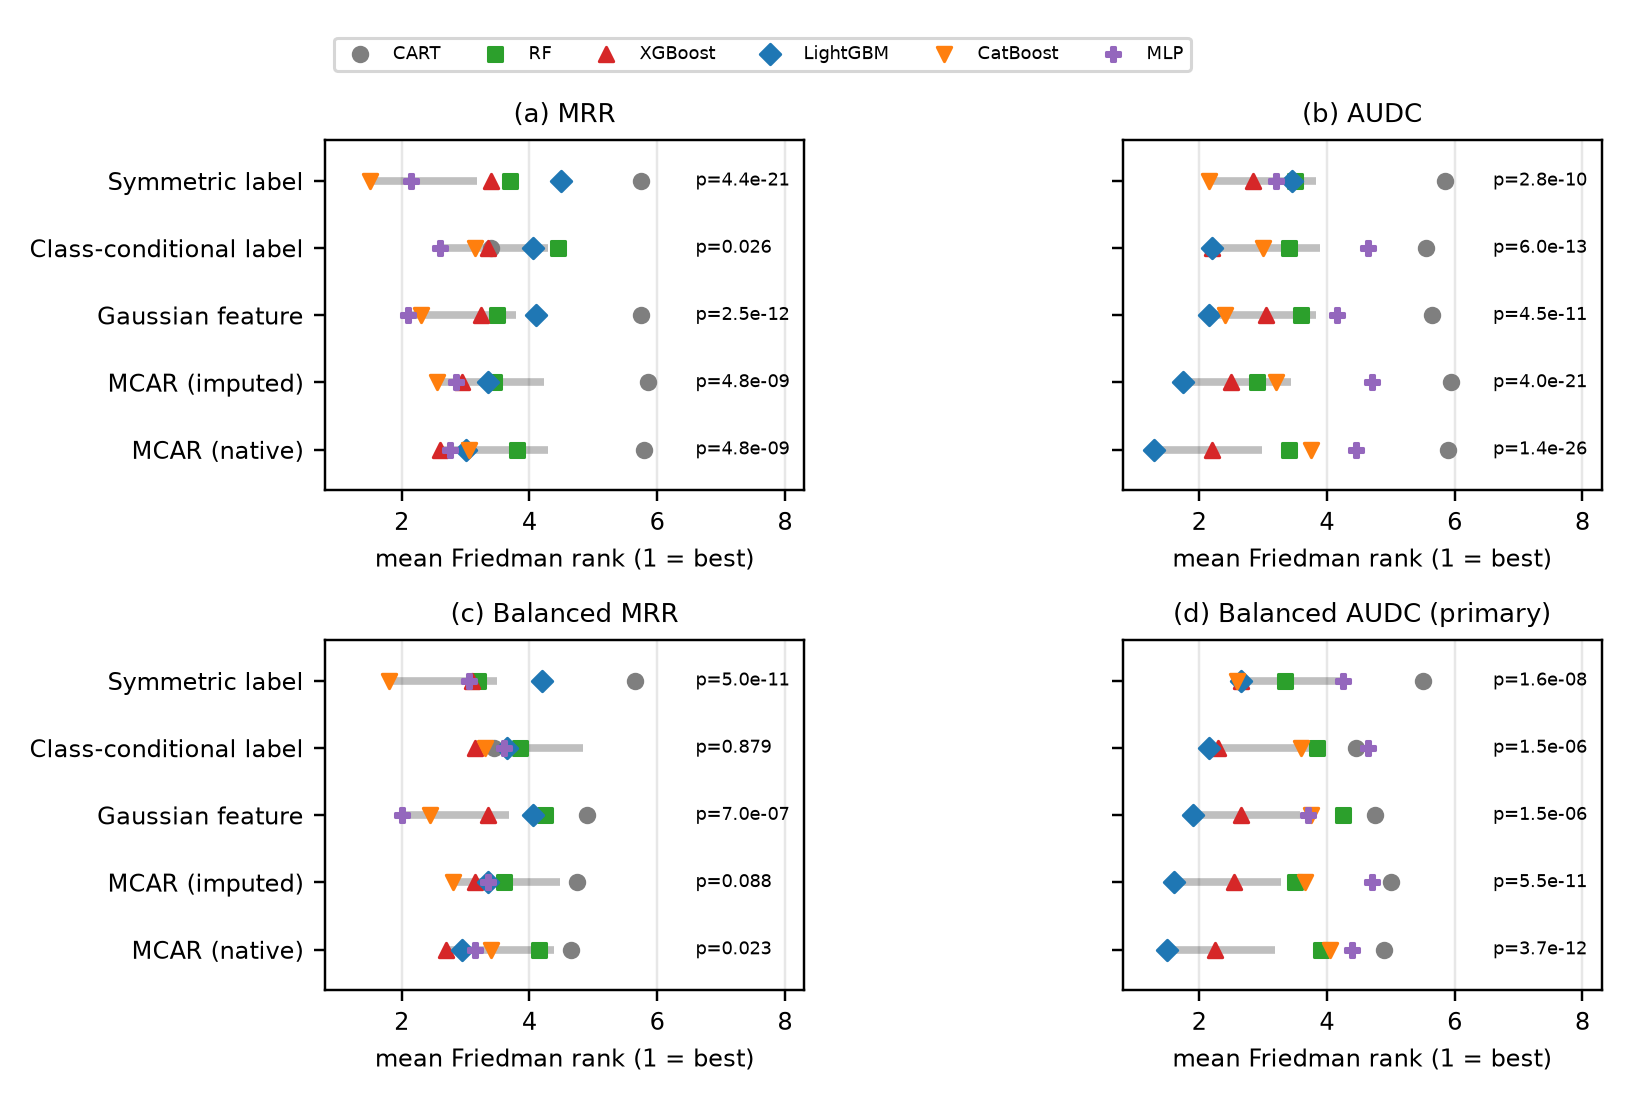
\includegraphics[width=0.75\linewidth]{fig_ranking.png}
\caption{Mean Friedman ranks of the six families under the five primary conditions (training robustness, Protocol~A, $N=20$): (a) MRR, (b) AUDC, (c) balanced MRR and (d) balanced AUDC, the primary measure. The grey bar starts at the best mean rank and has the length of the Nemenyi critical difference ($1.686$); models beyond it differ significantly from the best. $p$: Iman--Davenport, Holm-adjusted over the confirmatory family (a, b, d) or over all thirty tests (c).}
\label{fig:ranking}
\end{figure}

Each seed redraws the folds, the corruption and the model initialisation. Repeating the Friedman analysis seed by seed (Supplementary Table~S5), the best model is the same in all three seeds in 8 of 10 blocks of score and condition, and the smallest Kendall correlation between two seeds' mean-rank vectors is $0.60$. Within a single dataset, however, the margin between the two leading families is smaller than the seed-to-seed standard deviation of the leader's balanced AUDC in 35\% of the 100 dataset--condition blocks (margin: difference between the two leading families' seed-averaged balanced AUDC; standard deviation: across the three seeds for the leader; the earlier 48\% could not be reproduced under this definition): the identity of the best family on one dataset is often decided by the seed, whereas the rank tests, which pool twenty datasets, are not.

\subsection{Knee-estimator reliability and sensitivity}\label{sec:res:knee}

Curve-based robustness reporting often presupposes that a degradation trajectory has an operational inflection point that knee and elbow detectors~\cite{satopaa2011finding,salvador2004determining} can locate. This subsection audits that assumption for eleven-tier sweeps (RQ3). The answer is negative: the knee is not identifiable at this resolution, and it is reported as a caution, not as a TabStress measure.

\paragraph{Synthetic trajectories with known knees.} The synthetic results are a warning about the reliability of the estimator, not a validation of it. We sampled smoothed hinge trajectories with a known knee early ($0.10$), in the middle ($0.25$) or late ($0.40$) in the sweep, together with knee-free trajectories (linear, exponential and flat), at the eleven tiers, added Gaussian noise to each tier and applied the estimators 500 times per setting (Figure~\ref{fig:knee}a). Without noise the spline knee recovers every true knee to within $0.001$. At a noise level of $0.005$ per tier, about the standard error of a seed-averaged tier in our data, it recovers the knee within one tier in 89\%, 53\% and 26\% of replicates for early, middle and late knees, with a mean signed error of $-0.147$ for late knees, that is, towards earlier intensities. The reason is the curvature formula: $\kappa$ is damped by $(1+v^2)^{-3/2}$ on the steep segment after a knee, so noise on the flat segment before it wins. The discrete second-difference estimator, which uses the tiers directly, recovers all three within one tier in at least 82\% of replicates. Knee-free trajectories receive an interior knee from the spline estimator in 96\% of linear replicates, with a maximum curvature of the same size as that of true knees; at this noise level the magnitude of $\kappa$ cannot tell a knee from its absence.

\paragraph{Real trajectories.} On the benchmark data, 91\% of the 591 defined knees lie within $0.002$ of a sampled tier, as Supplementary Proposition~S2 predicts. Across seeds, the Spearman correlation of $\etaknee$ between two seeds is at most 0.26, and only 41\% of knees stay within one tier when the seed changes; the discrete estimator does better (Spearman up to 0.44, 46\% within one tier) but remains far from the endurance scores, whose seed-to-seed Spearman correlation is at least 0.98 for MRR and 1.00 for balanced AUDC (Figure~\ref{fig:knee}b). The original seed-42 design, which applied pair-flip noise to the binary datasets as well, produced two realizations of one corruption law on each of them (Proposition~\ref{prop:a_pairflip_binary}) that differ only in the noise draw: MRR replicates almost perfectly (Pearson $r=0.993$ over 84 pairs); the knee does not (Spearman $\rho=0.36$). A parametric bootstrap of the seed-averaged tiers gives a median 95\% interval width of 0.400 for $\etaknee$.

%% ---- begin inlined ../results/analysis/latex_primary/tab_ablation.tex ----
\begin{table}[t]
\centering
\small
\caption{Sensitivity of $\eta_{\mathrm{knee}}$ to the estimator, over all 600 seed-averaged trajectories. Each row is compared with the reference estimator (interpolating natural cubic spline, 11 tiers, $\arg\max\kappa$ on a 500-point grid), whose estimates are interior (Supplementary Proposition~S1): 0 of the 591 defined knees lie within $0.01$ of the boundary. ``Edge'' is the share of defined knees within $0.01$ of $0$ or $0.5$; trajectories with $\kappa\equiv0$ have no knee and are left out. The 500-point grid is a numerical search grid, not experimental resolution (11 tiers); read $\eta_{\mathrm{knee}}$ at tier level, as a secondary population-level descriptor.}
\label{tab:ablation}
\begin{tabular}{@{}p{4.3cm}rrrr@{}}
\toprule
Estimator & med.\ $\lvert\Delta\eta_{\mathrm{knee}}\rvert$ & $\le 0.05$ (\%) & Spearman & Edge (\%) \\
\midrule
Smoothing spline, $s=10^{-3}$, $\arg\max\lvert S''\rvert$ (legacy) & 0.200 & 1.5 & 0.22 & 100.0 \\
Interpolating cubic, not-a-knot ends & 0.014 & 56.7 & 0.73 & 40.6 \\
Natural cubic on 6 tiers ($\Delta\eta=0.10$) & 0.050 & 32.8 & 0.33 & 0.0 \\
Penalised cubic smoothing spline, GCV & 0.013 & 53.5 & 0.47 & 0.0 \\
\bottomrule
\end{tabular}
\end{table}
%% ---- end inlined ../results/analysis/latex_primary/tab_ablation.tex ----

\paragraph{Estimator sensitivity.} Table~\ref{tab:ablation} compares the reference estimator with four alternatives. A smoothing spline with argmax of $\lvert S''\rvert$, used in an earlier version of the pipeline, puts 100.0\% of knees on the boundary of the sweep; not-a-knot end conditions agree with the reference within one tier in 57\% of trajectories but send 42\% to the boundary; halving the number of tiers moves a knee by 0.050 in median; and a penalised smoothing spline flattens 14\% of trajectories to a nearly straight line, destroying the tier progression. The natural cubic spline interpolator on seed-averaged tiers avoids boundary artifacts while respecting tier measurements, but $\etaknee$ remains sensitive to estimator formulation, and Table~\ref{tab:ablation} is retained as an informative sensitivity demonstration.

\begin{figure}[t]
\centering
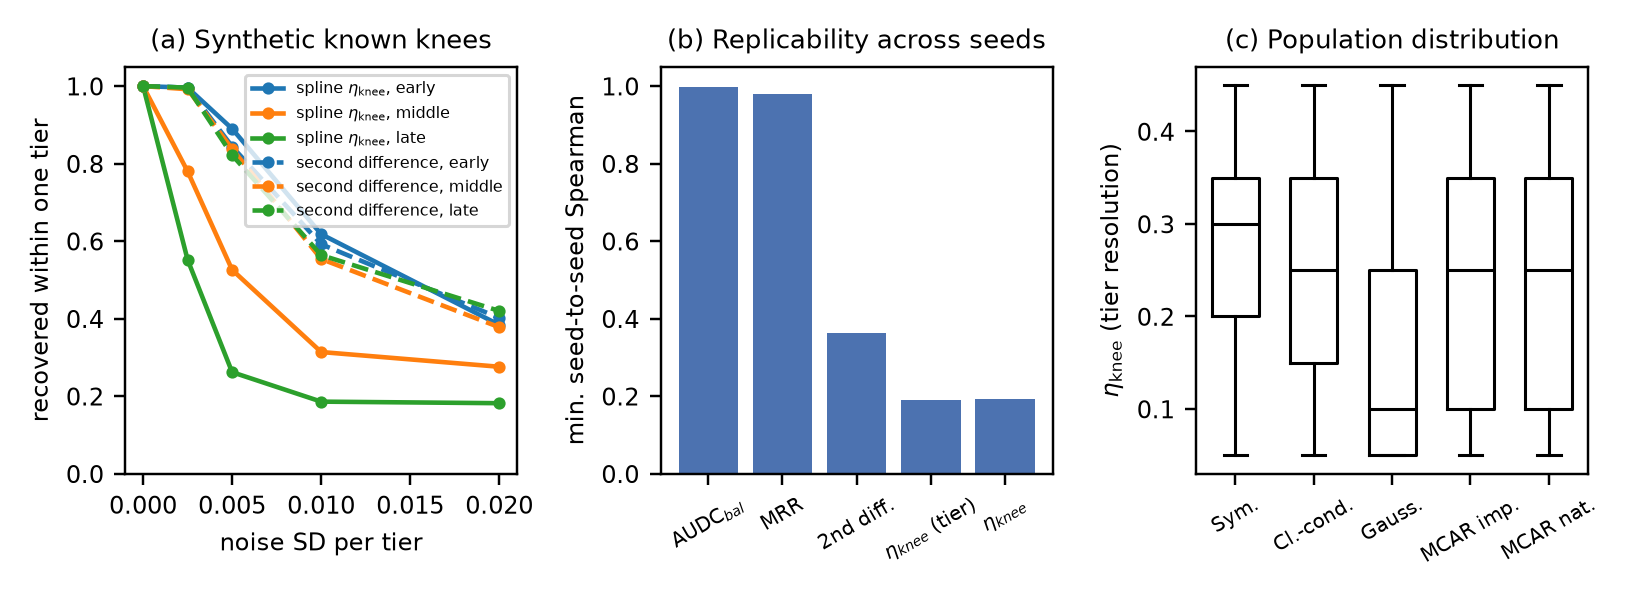
\includegraphics[width=0.75\linewidth]{fig_knee.png}
\caption{Reliability of the knee statistic. (a) Share of synthetic trajectories whose known knee is recovered within one tier, as a function of the noise added to each tier, for the spline estimator $\etaknee$ (solid) and the second-difference estimator (dashed). (b) Smallest seed-to-seed Spearman correlation over the three seed pairs, for the endurance scores and the knee estimators, on the 600 primary trajectories. (c) Distribution of $\etaknee$ at tier resolution over models and datasets, by condition.}
\label{fig:knee}
\end{figure}

\paragraph{What this means.} AUDC and MRR are reliable robustness descriptors: they replicate across seeds and noise draws, and the rankings in this article rest on them. $\etaknee$ is a secondary, population-level descriptive statistic; it is never a ranking criterion, and no result here says that a model fails at a particular intensity. The spline estimator is retained because it is the reference definition of the knee and its instability is itself a reported finding; the 500-point grid is a numerical search grid, not experimental resolution (eleven tiers), so knees are summarized at tier level. Pooled over models and datasets, the median knee lies at 0.10 under Gaussian noise (interquartile range $[0.05,0.30]$) and at 0.30 under symmetric label noise ($[0.20,0.35]$; Figure~\ref{fig:knee}c). Such a distribution is a coarse description of where a model family typically starts to deteriorate faster under a given operator. It is not an exact per-dataset failure point, and the knee of an individual trajectory should not be read on its own or used for deployment decisions.

\subsection{Ablation and configuration sensitivity}\label{sec:res:config}

\paragraph{Library defaults.} The matched budget treats the boosting libraries alike but is not how they ship (Supplementary Table~S7). CatBoost with 1{,}000 rounds and an automatically chosen learning rate gains clean accuracy (median $+0.0079$) and, under feature corruption, absolute endurance: its AUDC is higher on 18 of 20 datasets under Gaussian noise (Holm-adjusted $p=2.2\times10^{-4}$). Under symmetric label noise the larger budget cuts the other way and relative retention falls (median MRR change $-0.0172$). With every library at its defaults the AUDC leader under Gaussian noise is CatBoost instead of LightGBM.

\paragraph{Tuned configurations (exploratory).} On the twenty datasets of the tuning experiment, a six-trial search on clean data evaluates the sensitivity of rankings to mild hyperparameter tuning rather than seeking globally optimal models; it shows configuration sensitivity, not ranking stability under comprehensive tuning or under tuning for robustness. It changes the clean accuracy of the families by a median of between $+0.0003$ and $+0.0066$. Compared with the matched budget on the same folds and seed, the leading family is unchanged in three of the nine blocks of score and condition (symmetric label noise and Gaussian noise under Protocol~A, Gaussian noise under Protocol~B), and the smallest Kendall correlation between the matched and the tuned mean-rank vectors is $0.28$ (Table~\ref{tab:sensitivity}). The endurance scores themselves move little (largest median change $0.0061$), but the order of the leading families does (interpreted in Section~\ref{sec:disc:why}). The bottom of the ranking is more stable; CART is last under both configurations in six of the nine blocks.

\paragraph{Dataset artifacts.} We re-ran the primary protocol, all five conditions and three seeds, on the cleaned copies of spambase, churn and MiniBooNE defined in Section~\ref{sec:method:protocol} and, separately, repeated the rank tests without these three datasets and amazon\_access, on which two models are degenerate. Table~\ref{tab:sensitivity} summarizes both. Corrections and sensitivity runs are indexed with their scripts and summaries in PIPELINE\_MANIFEST.md (Section~5.4). With the cleaned copies substituted, the best model is unchanged in thirteen and the worst in fifteen of the fifteen confirmatory blocks, the smallest Kendall correlation with the reference mean-rank vectors is $0.87$, and all fifteen omnibus tests remain significant after Holm adjustment. Excluding the four flagged datasets leaves fourteen of fifteen tests significant at $N=16$ (smallest $\tau=0.71$). With the cleaned copies the principal conclusions are unchanged. Excluding the four flagged datasets changes the best model in four of the fifteen blocks (Table~\ref{tab:sensitivity}), so the conclusions survive the exclusion but the leaders do not.

Exact duplicate feature rows are present in five further datasets that the cleaned-copy analysis above does not cover: nomao (2,405 of 34,465 rows in the full upload, before the 10,000-row subsample), pol (42), volkert (12), phoneme (9) and ozone\_level (8). These counts are reproduced by \texttt{experiments/duplicate\_scan.py}. The primary grid retains these rows. Identical rows can fall into both training and evaluation folds, so the nomao accuracies in the primary grid may be inflated. For these five datasets we re-ran the primary protocol on cleaned copies (exact duplicates removed and feature vectors with conflicting labels dropped, before subsampling; seeds 42--44; all operators, including the multiclass pair-flip on pol and volkert). With the five cleaned copies substituted, the best model is unchanged in fifteen of fifteen confirmatory blocks, the worst model is unchanged in fifteen of fifteen, the smallest Kendall correlation with the reference mean-rank vectors is $0.83$, fourteen of fifteen omnibus tests remain significant after Holm adjustment, and no balanced-AUDC trajectory changes by more than $0.006$ (Table~\ref{tab:sensitivity}).

%% ---- begin inlined ../results/analysis/revision/tab_sensitivity.tex ----
\begin{table}[t]
\centering
\footnotesize
\caption{Sensitivity of the cross-model ranking. Each row compares the mean-rank vectors of a variant with the reference analysis over the fifteen confirmatory blocks (score $\times$ condition) or the stated blocks: blocks with the same best and worst model, the smallest Kendall $\tau$, and the number of omnibus tests that remain significant after Holm adjustment.}
\label{tab:sensitivity}
\begin{tabular}{@{}p{4.6cm}rrrr@{}}
\toprule
Variant & Same best & Same worst & min.\ $\tau$ & Significant \\
\midrule
Cleaned spambase, churn, MiniBooNE & 13/15 & 15/15 & $0.87$ & 15/15 \\
Flagged datasets excluded ($N=16$) & 11/15 & 14/15 & $0.71$ & 14/15 \\
Deduplicated nomao, pol, volkert, phoneme, ozone\_level & 15/15 & 15/15 & $0.83$ & 14/15 \\
Tuned instead of matched budget (seed 42) & 3/9 & 6/9 & $0.28$ & -- \\
\bottomrule
\end{tabular}
\end{table}
%% ---- end inlined ../results/analysis/revision/tab_sensitivity.tex ----


\subsection{Inference robustness (Protocol~B)}\label{sec:res:deploy}

Protocol~B answers a different question from Protocol~A: does a model trained on clean data keep its accuracy when its inputs deteriorate? Table~\ref{tab:protocol} compares the two protocols on the conditions they share, and Figure~\ref{fig:overall} (bottom) shows balanced AUDC for inference robustness; Supplementary Table~S8 gives the omnibus tests of all 42 Protocol~B blocks, of which 38 reject equal mean ranks after Holm adjustment.

%% ---- begin inlined ../results/analysis/revision/tab_protocol.tex ----
\begin{table*}[t]
\centering
\footnotesize
\caption{Training robustness (Protocol~A, corrupted training and test data) against inference robustness (Protocol~B, clean training, corrupted test data) on matched conditions. $\Delta$: median over the 120 dataset--model pairs of the score under B minus the score under A (negative values indicate performance degradation under deployment corruption); B$<$A: share of pairs with a lower score under B; $p$: Wilcoxon signed-rank test of the paired differences; leaders: model with the lowest mean rank under A / B; $\tau$: Kendall correlation of the two mean-rank vectors (smaller values indicate greater reordering of the ranking between the two protocols). Upper block: seeds 42--44, twenty datasets; lower block: seeds 42--44, the same twenty datasets, for both protocols.}
\label{tab:protocol}
\begin{tabular}{@{}llrrrlr@{}}
\toprule
Condition & Score & $\Delta$ (B$-$A) & B$<$A (\%) & $p$ & Leader A / B & $\tau$ \\
\midrule
Gaussian & AUDC$_{\mathrm{bal}}$ & $-0.0001$ & 50 & 0.051 & LightGBM / MLP & $0.14$ \\
 & AUDC & $-0.0058$ & 75 & $1.6\times10^{-10}$ & LightGBM / RF & $0.20$ \\
 & MRR & $-0.0076$ & 74 & $1.4\times10^{-10}$ & MLP / MLP & $0.87$ \\
MCAR, imputed & AUDC$_{\mathrm{bal}}$ & $-0.0062$ & 62 & 0.006 & LightGBM / LightGBM & $1.00$ \\
 & AUDC & $-0.0063$ & 70 & $1.5\times10^{-6}$ & LightGBM / RF & $0.60$ \\
 & MRR & $-0.0067$ & 69 & $4.0\times10^{-6}$ & CatBoost / MLP & $0.60$ \\
MCAR, native & AUDC$_{\mathrm{bal}}$ & $-0.0037$ & 55 & 0.007 & LightGBM / RF & $0.20$ \\
 & AUDC & $-0.0109$ & 62 & $1.1\times10^{-6}$ & LightGBM / RF & $0.07$ \\
 & MRR & $-0.0115$ & 62 & $3.3\times10^{-6}$ & XGBoost / RF & $-0.47$ \\
\midrule
MAR, imputed & AUDC$_{\mathrm{bal}}$ & $-0.0064$ & 65 & $2.4\times10^{-4}$ & LightGBM / LightGBM & $1.00$ \\
 & AUDC & $-0.0058$ & 68 & $1.0\times10^{-7}$ & LightGBM / LightGBM & $0.73$ \\
 & MRR & $-0.0067$ & 68 & $3.0\times10^{-7}$ & CatBoost / CatBoost & $0.73$ \\
MNAR, imputed & AUDC$_{\mathrm{bal}}$ & $-0.0072$ & 62 & $1.7\times10^{-5}$ & LightGBM / LightGBM & $0.87$ \\
 & AUDC & $-0.0100$ & 77 & $6.5\times10^{-10}$ & LightGBM / LightGBM & $0.87$ \\
 & MRR & $-0.0120$ & 77 & $1.7\times10^{-9}$ & XGBoost / CatBoost & $0.33$ \\
\bottomrule
\end{tabular}
\end{table*}
%% ---- end inlined ../results/analysis/revision/tab_protocol.tex ----

\paragraph{Scores are lower and rankings change.} Under clean training the endurance scores are lower than under corruption-aware training in 8 of the 9 matched blocks (Wilcoxon $p<0.05$) and never significantly higher: a learner that is refitted on corrupted data adapts to it, and Protocol~A therefore overstates the robustness of a deployed model. The median losses are small in absolute terms, about one point of accuracy, but the order of the families moves: the leading family is the same under both protocols in only two of the nine blocks, and the median Kendall correlation between the two mean-rank vectors is $0.20$ (minimum $-0.47$). Under Gaussian noise the MLP, whose decision function is smooth in its inputs, leads on balanced AUDC, while the tree ensembles, whose split thresholds were fitted to clean values, lose more; under imputed masking LightGBM keeps the lead on balanced AUDC under MCAR, MAR and MNAR alike.

\paragraph{Native missing-value handling reverses.} The sharpest change concerns missing values. Because the boosters are trained on clean folds that contain no missing values, they have no data from which to learn a split-routing direction for one; native handling then acts as an uncalibrated default at deployment, and degrades performance unless it is paired with imputation. This is a finding about deployment pipelines, not about native handling as such: under Protocol~A, where missing values are present during training, native handling made no material difference (Section~\ref{sec:res:feature}). Under deployment masking, native handling lowers the AUDC of all three boosters relative to median imputation in 8 of nine family--mechanism tests (Holm-adjusted $p<0.05$); for XGBoost under MCAR the median loss is $-0.051$ and AUDC is lower on 100\% of datasets. CART and the random forest, whose scikit-learn implementation sends missing values to the child that received more training samples, gain instead (median $+0.009$ for the forest under MCAR). As a result the random forest leads on every score under every native-handling condition of Protocol~B, and XGBoost or CatBoost is last on balanced AUDC, whereas under Protocol~A native handling made no material difference (Section~\ref{sec:res:feature}).

\paragraph{Clean accuracy at deployment.} The negative answer to RQ1 holds under deployment corruption: the most accurate clean model is also the one with the highest MRR in at most 10\% of datasets under any Protocol~B condition.

\paragraph{The TabICL baseline.} TabICL (Section~\ref{sec:method:models}), an exploratory, secondary, inference-time baseline, was evaluated under Protocol~B on nineteen datasets with seeds 42, 43 and 44, sharing the folds and corruption draws of the classical families, but not under an equal compute or configuration budget (Table~\ref{tab:foundation}). TabICL was evaluated under a constrained setting (an ensemble of four estimators instead of eight, in-context set capped at 3{,}000 rows) to bound inference cost. It is a secondary analysis, and the Holm adjustment covers the twelve tests of this block. On the nineteen TabICL datasets, TabICL has the highest mean clean accuracy ($0.880$, against $0.848$ for the best classical family on the same datasets) and the best mean clean rank among the seven (2.05), and it is the most accurate clean model on ten of the nineteen datasets. That advantage carries into the absolute scores mainly under imputed masking. Under MCAR and MAR masking TabICL ranks first or second of the seven on both balanced AUDC and AUDC, although its median difference from the best classical family stays within $0.006$ in absolute value under both mechanisms on both scores. Under MNAR masking classical families lead both scores, LightGBM on balanced AUDC, and under Gaussian feature noise TabICL falls to mean rank 4.89 on balanced AUDC, where the MLP leads (2.84), with a median difference of $-0.065$. On the relative score the order reverses. TabICL ranks sixth or seventh on MRR under every operator (mean rank 5.05 to 5.68), is last under two of the four, and exceeds the best classical family on MRR on at most 11\% of the datasets under any operator. Adding it to the pool leaves the order of the six classical families essentially unchanged (Kendall $\tau\ge0.97$ in all twelve blocks). The negative answer to RQ1 also stands with seven models: the most accurate clean model is the most robust by MRR in 4\% of dataset--operator blocks, averaged over the four operators, and by balanced AUDC on 43\% (43\% with the six classical families). Bootstrap 95\% intervals over datasets for the median MRR difference between TabICL and the best classical family lie below zero under every operator (largest upper limit $-0.006$). Table~\ref{tab:tabicl_configs} separates the constrained main configuration from a default-setting sensitivity run on six datasets and one seed (eight estimators, no cap on the in-context set); the two runs have different compute budgets and are not an equal-budget comparison. The MRR mean rank of TabICL and its clean accuracy (within $0.013$) are unchanged to two decimals; the per-dataset MRR values are not identical (they differ by up to 0.07, the per-dataset table in the Supplementary Material), so the equal mean ranks reflect the ordering among seven models rather than identical inputs, whereas its balanced-AUDC rank under MNAR masking rises from 3.67 to 2.83, so the absolute scores of the main run may understate TabICL on this subset; with six datasets and one seed this shift is descriptive and untested (Supplementary Section~S9). The clean-accuracy lead and the weaker relative retention describe this one model under these constrained settings and one protocol; they are not evidence about tabular foundation models as a class.

%% ---- begin inlined ../results/analysis/revision/tab_tabicl_configs.tex ----
\begin{table}[t]
\centering
\footnotesize
\caption{TabICL, secondary analysis (inference robustness, Protocol~B, seed 42, 6 datasets): constrained main configuration (4 estimators, in-context set capped at 3,000 rows) against a default-setting sensitivity run (8 estimators, no cap). The two runs use different compute budgets and are not an equal-budget comparison; the default run covers a subset of datasets and one seed. Mean rank of TabICL among the seven models (position in parentheses). Unchanged: TabICL's MRR rank under all four operators and its clean accuracy. Changed: its balanced-AUDC rank under MNAR masking. No claim extends to foundation models as a class.}
\label{tab:tabicl_configs}
\begin{tabular}{@{}llrr@{}}
\toprule
Score & Operator & Main (constrained) & Default \\
\midrule
MRR & Gaussian & 6.83 (7) & 6.83 (7) \\
 & MCAR & 5.33 (6) & 5.33 (6) \\
 & MAR & 5.17 (6) & 5.17 (6) \\
 & MNAR & 5.17 (7) & 5.17 (7) \\
\midrule
AUDC$_{\mathrm{bal}}$ & Gaussian & 5.00 (6) & 5.00 (6) \\
 & MCAR & 2.33 (1) & 2.00 (1) \\
 & MAR & 1.83 (1) & 1.67 (1) \\
 & MNAR & 3.67 (5) & 2.83 (1) \\
\midrule
Clean accuracy (mean) & -- & 0.935 & 0.938 \\
\bottomrule
\end{tabular}
\end{table}
%% ---- end inlined ../results/analysis/revision/tab_tabicl_configs.tex ----

%% ---- begin inlined ../results/analysis/revision/tab_foundation.tex ----
\begin{table}[t]
\centering
\footnotesize
\caption{The pretrained TabICL baseline among the six classical families under Protocol~B (inference robustness; clean in-context training set, corrupted evaluation, imputed pipeline, seeds 42, 43, 44, $N=19$ datasets). Mean Friedman rank of TabICL among the seven models and the model with the lowest mean rank (rank in parentheses); adj.\ $p$: Iman--Davenport $p$-value of the seven-model comparison, Holm-adjusted over the twelve tests of the block; $\Delta$: median over datasets of TabICL's score minus that of the best classical family. Secondary analysis; TabICL was run under a constrained configuration and the table does not generalize to foundation models as a class.}
\label{tab:foundation}
\begin{tabular}{@{}llrlrr@{}}
\toprule
Score & Operator & TabICL rank & Leader of seven & adj.\ $p$ & $\Delta$ \\
\midrule
Clean accuracy & -- & 2.05 & TabICL (2.05) & -- & $+0.001$ \\
\midrule
AUDC$_{\mathrm{bal}}$ & Gaussian & 4.89 & MLP (2.84) & 0.003 & $-0.065$ \\
 & MCAR & 2.63 & LightGBM (2.61) & $4.6\times10^{-6}$ & $-0.006$ \\
 & MAR & 2.37 & TabICL (2.37) & $1.3\times10^{-6}$ & $-0.005$ \\
 & MNAR & 2.95 & LightGBM (2.61) & $6.3\times10^{-6}$ & $-0.006$ \\
\midrule
AUDC & Gaussian & 4.00 & CatBoost (2.71) & $9.7\times10^{-7}$ & $-0.032$ \\
 & MCAR & 2.58 & TabICL (2.58) & $1.1\times10^{-14}$ & $-0.001$ \\
 & MAR & 2.37 & TabICL (2.37) & $4.5\times10^{-16}$ & $0.000$ \\
 & MNAR & 3.16 & LightGBM (2.76) & $4.6\times10^{-15}$ & $-0.006$ \\
\midrule
MRR & Gaussian & 5.68 & MLP (1.79) & $7.2\times10^{-16}$ & $-0.093$ \\
 & MCAR & 5.05 & MLP (2.74) & $3.5\times10^{-5}$ & $-0.021$ \\
 & MAR & 5.05 & CatBoost (2.66) & $3.0\times10^{-4}$ & $-0.019$ \\
 & MNAR & 5.42 & CatBoost (2.82) & $2.9\times10^{-4}$ & $-0.023$ \\
\bottomrule
\end{tabular}
\end{table}
%% ---- end inlined ../results/analysis/revision/tab_foundation.tex ----

The answer to the question that motivated Protocol~B is therefore that the two protocols measure different properties. Corruption-aware training measures how well a learning procedure copes with a persistently degraded measurement process; inference robustness measures how a trained model copes with inputs that deteriorate after training. Both are reported, and only the second supports claims about deployed models.


%% ===========================================================================
\section{Discussion}\label{sec:discussion}

\subsection{Main findings}\label{sec:disc:findings}

Three findings carry the article. First, clean-data performance does not reliably predict robustness under data corruption: within a dataset the most accurate clean model is rarely the one that retains the largest share of its accuracy, and only about half the time the one with the highest balanced AUDC (Section~\ref{sec:res:overall}). Second, robustness rankings depend on the corruption mechanism, the evaluation metric, the model configuration and the evaluation protocol (Sections~\ref{sec:res:label} to~\ref{sec:res:deploy}). Third, curve-level endurance scores are reliable descriptors, whereas the knee of a trajectory is not identifiable at standard sweep resolution, a caution for any robustness study that reports inflection points (Section~\ref{sec:res:knee}). Balanced AUDC is the primary outcome; MRR and aMRR are complementary views, and aMRR is uninformative when a model has almost no above-baseline skill.

The statistical evidence separates three levels. Whether rankings differ across datasets is answered by the omnibus tests: mean ranks differ under all fifteen confirmatory tests after Holm adjustment. Which models differ is answered by the pairwise tests, which separate only some pairs (Table~\ref{tab:combined}, Pairs). How large the differences are in practice is answered by effect sizes: Kendall's $W$ is only $0.12$ to $0.76$, and the two leading families are practically equivalent, with a median gap below one point of balanced AUDC and the $\pm0.01$ region of practical equivalence the most probable outcome in five of five conditions (Supplementary Section~S9). A significant omnibus result is therefore not evidence of a practically meaningful ordering.

\subsection{Why rankings change}\label{sec:disc:why}

The operators explain much of what the curves show. We conjecture, without testing it directly, that symmetric label noise leaves the Bayes classifier in place and costs sample efficiency, which would favor learners that average many weak fits; class-conditional noise moves the decision rule that every learner estimates, so the dataset matters more than the model and accuracy is retained by drifting towards the majority class. Budget explains the booster ordering: the matched 100-round budget favors learners that converge quickly, and at its 1{,}000-round default CatBoost overtakes LightGBM under Gaussian noise; under symmetric label noise the extra rounds fit the corrupted labels and lower relative retention. Under feature corruption we conjecture that the absolute and the relative view diverge because capacity and graceful degradation are different properties: a model that fits fine structure in clean data gains accuracy at $\eta=0$ and has more to lose when that structure is blurred. The protocol changes the question itself. Under corruption-aware training a learner re-estimates its splits or weights on corrupted inputs at every intensity; a model trained on clean data meets inputs it has never seen. Missing values are a plausible case: a booster that has seen no missing value during training may have no learned direction for one, and its native routing at deployment is an arbitrary default rather than an estimate, whereas median imputation maps the missing entry to a typical value that the model has seen. The pretrained model illustrates the same divergence between capacity and graceful degradation: TabICL starts from the highest clean accuracy and ranks first or second on the absolute scores under MCAR and MAR masking, yet it ranks sixth or seventh of seven on retention (MRR) under every deployment operator (Section~\ref{sec:res:deploy}). One model under constrained settings cannot separate a property of pretraining from a property of this model, and nothing here generalizes to foundation models as a class. Configuration matters for similar reasons, because the number of boosting rounds and the learning rate decide how much fine structure is fitted. Interpreting the tuning and library-default runs, which family is most robust depends on the configuration (configuration robustness) and not only on the family (model-family robustness). Because the tuned runs use a six-trial clean-data random search on one seed, they show configuration sensitivity, not ranking stability under comprehensive or robustness-targeted tuning, and the data separate the two only within the three configuration regimes tested.

\subsection{Practical implications}\label{sec:disc:practice}

The evidence supports four qualified implications; they are findings of this controlled benchmark, not predictions that a ranking on twenty datasets transfers to a production system. They derive from twenty public datasets, six model families, synthetic stochastic corruption and three configuration regimes:
\begin{enumerate}
\item \emph{Evaluate under the protocol that matches deployment.} When production feeds deteriorate after model deployment, inference robustness (Protocol~B) is the relevant estimand; in this benchmark Protocol~A gave higher scores in eight of nine matched blocks and the same leading family in only two. The two protocols estimate different quantities, so this compares which protocol's score is more favorable on matched blocks; it is not evidence that one protocol is the more correct estimand.
\item \emph{Report balanced absolute and relative scores with baseline verification.} Clean accuracy does not identify robust models. Absolute endurance ($\AUDC_{\mathrm{bal}}$) identifies the highest performers on degraded data; relative retention ($\MRR$) and baseline-adjusted retention ($\aMRR$) add a second view of the same curves.
\item \emph{Align missing-value handling with where missingness occurs.} Here native routing gave no advantage over median imputation when missingness was present in training, and lowered the AUDC of the gradient boosters in eight of nine tests (native minus median imputation under Protocol~B; median loss up to 0.051 for XGBoost under MCAR, with native routing lower on every dataset) when it appeared only at deployment.
\item \emph{Treat hyperparameter configurations as an integral part of the model.} Report the configuration with the ranking. Within the three regimes tested, rankings shifted under a six-trial clean-data search and under library defaults; stability under thorough or corruption-targeted tuning is untested, so model-family superiority cannot be separated from configuration choices here.
\end{enumerate}
Using $\etaknee$ to calibrate production alarms is future work: it would require validation of thresholds, false-positive and false-negative rates, and real drift, none of which is provided here. The benchmark is not direct evidence of real-world deployment robustness; validation on a dataset with naturally occurring missingness or documented measurement errors is needed.

\subsection{Comparison with existing robustness measures}\label{sec:disc:measures}

AUDC is the accuracy analogue of the mean corruption error of Hendrycks and Dietterich~\cite{hendrycks2019benchmarking}, averaged over a dense sweep of one operator rather than a few severities of many, and without a reference model; MRR corresponds to a relative corruption error normalized by the model's own clean performance, and the equalized loss of accuracy of S\'aez et al.~\cite{saez2015evaluating} combines the two views in one number. Our results argue against collapsing them: AUDC and MRR name different leading families under four of the five primary conditions, and the baseline-adjusted ratio shows when a relative lead is real and when it is an effect of a low starting point. Effective robustness under distribution shift~\cite{taori2020measuring} similarly measures performance relative to a baseline trend. What TabStress adds to these measures is the response curve as the unit of analysis, the separation of training-time and deployment-time corruption, and a designated cross-dataset test of the resulting rankings.

\subsection{Limitations}\label{sec:disc:limits}

The corruptions are synthetic, stochastic and applied one at a time; real data deteriorate through several mechanisms at once and sometimes adversarially. A compound run on six datasets (label or Gaussian noise together with MCAR missingness at the same intensity) lost less accuracy than the sum of the two single-operator losses: the median difference between the compound AUDC loss and that sum was $-0.019$ for label noise and $-0.002$ for Gaussian noise, so negative values indicate sub-additive loss and kept the MRR order of the noise component (Kendall $\tau\ge0.96$) but not that of the missingness component ($\tau$ as low as 0.28; Supplementary Section~S9). The confirmatory claims are limited to classical supervised tabular learners trained from scratch. One tabular foundation model, TabICL, is covered as a secondary analysis under Protocol~B only, on nineteen datasets, with an ensemble of four, an in-context set of at most 3{,}000 rows and imputed inputs; it was not run under corruption-aware training, and no other foundation model was run. The tuned configurations come from a six-trial search on clean data and use one seed on all twenty datasets; the Protocol~A runs of the MAR and MNAR operators cover all twenty datasets and use three seeds; the categorical operators can be studied only on the six datasets with nominal attributes. All datasets are public and curated, and Section~\ref{sec:threats} discusses the remaining threats.


%% ===========================================================================
\section{Threats to Validity}\label{sec:threats}

\subsection{Benchmark selection bias}\label{sec:threats:selection}
Twenty public OpenML datasets, most of them members of curated suites, are not a random sample of operational tables: they are clean, mostly medium-sized and repeatedly studied. The selection criteria are explicit (Section~\ref{sec:method:protocol}), the cleaned-data and exclusion analyses of Section~\ref{sec:res:config} show that the rankings do not hinge on the three datasets with documented artifacts (spambase, churn and MiniBooNE); the duplicate-row contamination of the other five datasets is treated separately below, and the rank tests treat datasets as the unit of inference. Enterprise, streaming or uncurated industrial data may still behave differently.

\subsection{Synthetic corruption realism}\label{sec:threats:realism}
All corruptions are synthetic, stochastic and independent of any causal structure among the features. The all-column Gaussian variant perturbs one-hot indicators and ordinal codes as if they were measurements, so it is not a universal model of sensor degradation; the principal Gaussian condition applies the noise to continuous attributes only (Table~\ref{tab:gaussian_principal}), and the categorical-aware and categorical-only operators treat the nominal attributes recorded in the OpenML metadata on the six datasets that have any. The MAR and MNAR operators are rank-based stylisations of informative missingness, not models of a particular domain. Worst-case and adversarial corruption are outside the design.

\subsection{Hyperparameter sensitivity}\label{sec:threats:hyper}
The benchmark compares fixed inductive biases under standardized configurations rather than hyperparameter-optimized frontiers. Bayesian search across all tiers and deep tabular architectures such as FT-Transformer~\cite{gorishniy2021revisiting} are left to future work; the MLP results represent a classical dense baseline, not modern deep architectures. The matched budget, library defaults and a six-trial random search on all twenty datasets are three points in a large configuration space. Section~\ref{sec:res:config} shows that configuration changes the leading booster under feature corruption; a more thorough search, or tuning under corruption, could reorder the families further. Rankings in this article are rankings of configured pipelines, and the distinction between model-family and configuration robustness is drawn only as far as these three regimes allow. TabICL was run with one configuration (defaults apart from ensemble size and context cap); its ranking relative to classical families could change with the full ensemble.

\subsection{Metric-induced ranking bias}\label{sec:threats:metric}
Every score encodes a question, and the rankings differ between scores (Section~\ref{sec:res:absrel}). Fixing the roles of the scores before the tests, reporting balanced and baseline-adjusted versions and controlling the confirmatory family jointly limit, but do not remove, the influence of the choice of score. Intensities are not comparable across operators, so no statement in this article ranks corruption types by harm.

\subsection{Model-version dependence}\label{sec:threats:version}
Results are tied to scikit-learn 1.9.1, XGBoost 3.4.1, LightGBM 4.7.0 and CatBoost 1.2.10, and those for the pretrained model to tabicl 2.2.0 with its default checkpoint and torch 2.14.1 (TabICL results describe that version under the constrained configuration of Section~\ref{sec:method:models} only), whose floating-point arithmetic is subject to standard hardware platform differences. Defaults, histogram binning and missing-value routing change between library versions; the pinned environment in the replication package reproduces stored cells exactly, but a different version can change individual cells and, near ties, mean ranks.

\subsection{Temporal reproducibility of external datasets}\label{sec:threats:temporal}
OpenML datasets are addressed by stable identifiers, but uploads can be deprecated or re-processed. The replication package caches the exact matrices used, and the ten-thousand-row subsample is fixed by seed, so the experiment does not depend on the future state of the repository. The subsample of the nine datasets with more than 10{,}000 rows was drawn once, with seed 42; alternative subsamples were not evaluated, so subsampling variance is not part of the reported seed variation.

\subsection{Computational-budget bias}\label{sec:threats:budget}
The matched-budget comparison is confounded with boosting rounds and is a configuration comparison, not a measure of intrinsic family robustness (Section~\ref{sec:disc:why}). The ten-thousand-row cap, five folds and three seeds bound compute and resolution: on the smallest dataset a single cell cannot detect an accuracy gap of $0.02$ reliably, and claims rest on cross-dataset rank tests. TabICL was evaluated under constrained settings (Protocol~B only, four estimators, $\le 3{,}000$ context rows, Bioresponse excluded) due to compute limits; its scores describe this configuration, not an attainable bound, and confirmatory conclusions remain those for the six classical families.

\subsection{Internal validity}\label{sec:threats:internal}
Corruptions are applied inside the cross-validation folds, labels are scored against clean targets, and every random stream is seeded and audited (Section~\ref{sec:method:engine}). Numerical verification confirms exact reproducibility across seeds, with recomputation audits validating the stored evaluation cells. Fold standard deviations understate the variability of cross-validation because folds share training data; the seed replication of Section~\ref{sec:res:stats} addresses this for the endurance scores. The dataset artifacts defined in Section~\ref{sec:method:protocol} are re-run in Section~\ref{sec:res:config}, where removing them leaves the best and worst model unchanged in all fifteen confirmatory blocks. Corrections and sensitivity runs are indexed with their scripts and summaries in PIPELINE\_MANIFEST.md (Section~5.4).

%% ===========================================================================
\section{Conclusion}\label{sec:conclusion}

TabStress is a controlled evaluation design that profiles tabular classifier degradation under stochastic, non-adversarial corruption. It does not claim novelty for any single component; its contribution is the combination of corruption-response curves, absolute and relative endurance measures, cross-dataset rank testing and a qualified knee descriptor. It keeps two estimands apart: Protocol~A measures the robustness of a learning procedure under a persistently corrupted data-generating process, and Protocol~B measures the robustness of a trained model to deteriorating evaluation inputs.

For practitioners, clean accuracy is not a sufficient proxy for robustness, and any robustness claim should name its corruption mechanism, metric, configuration and protocol. No family dominates under these settings: the best family differs by corruption and metric, and balanced relative retention ($\MRR_{\mathrm{bal}}$) under class-conditional label noise does not distinguish the families. TabICL is one pretrained model under constrained settings and one protocol, and its results are not generalized to foundation models.

Curve-level endurance scores are seed-replicable summaries, with $\AUDC_{\mathrm{bal}}$ primary. The knee $\etaknee$ is unstable on individual trajectories and serves only as a secondary, coarse population-level descriptor, never as a failure threshold.

These findings come from a controlled synthetic-corruption benchmark on twenty datasets and are not direct evidence of real-world deployment robustness. Future work should validate the protocols on data with naturally occurring missingness or documented measurement errors, extend profiling to other foundation models and compound corruptions, and test any monitoring use of the knee against false-alarm rates.


\backmatter

\section*{Declarations}\label{sec:declarations}

\bmhead{Ethical Approval}
Not applicable. This study does not involve human participants, animal subjects, or sensitive personal data. All experiments were conducted on publicly available OpenML datasets.

\bmhead{Consent to participate and publish}
Not applicable. This study does not involve human participants.

\bmhead{Materials availability}
Not applicable. No physical materials were used.

\bmhead{Competing interests}
The authors declare no competing financial or non-financial interests.

\bmhead{Funding}
No external funding was received for conducting this study.

\bmhead{Authors' contributions}
S.M.S. supervised the research, formulated the study scope, and reviewed the manuscript. D.P. designed the benchmarking architecture, implemented the code, conducted the mathematical derivations, analyzed the empirical results, and wrote the manuscript. Both authors reviewed and approved the final manuscript.

\bmhead{Acknowledgments}
The authors thank the School of Computer Science and Engineering, Vellore Institute of Technology, and the maintainers of OpenML and of the benchmark datasets. The use of automated language tools is described in Section~\ref{sec:method:protocol}.

\bmhead{Data Availability}
All datasets are publicly available on OpenML under the identifiers listed in Supplementary Table~S2. The complete pre-computed cell matrices, seed replications, and cached datasets are available to reviewers now in the replication repository \url{https://github.com/RaffeOP/TabStress}, which also contains a manifest mapping each main table and figure to the files that generate it; a Zenodo DOI will be minted for the accepted version.

\bmhead{Code Availability}
The complete software implementation, including the corruption engine, evaluation harnesses for Protocol~A and Protocol~B, spline and knee estimation routines, statistical testing scripts, and manuscript reproduction pipelines, is available to reviewers now in the replication repository \url{https://github.com/RaffeOP/TabStress}; a Zenodo DOI will be minted for the accepted version.

\bmhead{Supplementary Material}
The label-noise derivations are given in Appendix~\ref{app:math}; the operator and knee-estimator derivations are in Supplementary Section~S1. The Supplementary Material contains detailed corpus, search-space, per-seed, native-handling, library-default and Protocol~B tables (Section~S2), per-condition critical-difference diagrams (Section~S3), per-dataset endurance (Section~S4), trajectory summaries with bootstrap intervals (Section~S5), the complete accuracy grid (Section~S6), the degradation atlas (Section~S7), pairwise Wilcoxon tests (Section~S8), sensitivity runs (Section~S9), and the data-cleaning rules with the pol class-ordering sensitivity analysis (Section~S10).

%% ===========================================================================
\renewcommand{\bibfont}{\footnotesize}\setlength{\bibsep}{0pt}
\bibliography{TabStress}

\begin{appendices}

\section{Mathematical derivations}\label{app:math}
This appendix derives the label-noise properties that Section~\ref{sec:problem} relies on and interprets them for the metrics. The secondary derivations (Gaussian and MCAR operators, natural-spline interior-knee and knot-extremum properties) are in Supplementary Section~S1 (Propositions~S1--S4).

Notation follows Section~\ref{sec:problem}: $p_k(\mathbf{x})$ and $\tilde p_k(\mathbf{x})$ are the clean and corrupted class posteriors, $\eta\in[0,0.5]$ the intensity.

\begin{appproposition}[Symmetric noise attenuates without moving the Bayes classifier]\label{prop:a_symmetric}
Under symmetric label noise $\tilde{p}_k(\mathbf{x})=\bigl(1-\frac{K\eta}{K-1}\bigr)p_k(\mathbf{x})+\frac{\eta}{K-1}$. For $\eta<(K-1)/K$ the Bayes classifier of the noisy problem coincides with that of the clean problem; at $\eta=(K-1)/K$ the noisy label is independent of $\mathbf{X}$.
\end{appproposition}
\begin{proof}
$\tilde{p}_k=(1-\eta)p_k+\sum_{j\ne k}p_j\,\eta/(K-1)=(1-\eta)p_k+(1-p_k)\eta/(K-1)$, which rearranges to the stated form. The map is affine with slope $1-K\eta/(K-1)$, positive for $\eta<(K-1)/K$, so it preserves the order of the $p_k$ and hence the argmax. The slope vanishes at $\eta=(K-1)/K$, leaving $\tilde{p}_k\equiv 1/K$.
\end{proof}

\begin{appproposition}[Pair-flip and symmetric noise coincide when $K=2$]\label{prop:a_pairflip_binary}
For $K=2$ the pair-flip and symmetric operators have the same transition matrix $\bigl(\begin{smallmatrix}1-\eta&\eta\\ \eta&1-\eta\end{smallmatrix}\bigr)$.
\end{appproposition}
\begin{proof}
With two classes, $(k+1)\bmod 2$ is the only other class, which symmetric noise also selects with probability $\eta/(K-1)=\eta$.
\end{proof}
The seed-42 runs of the original design applied pair-flip noise to every dataset; on the binary datasets they are therefore a second realization of symmetric noise and serve as a natural test--retest pair (Section~\ref{sec:res:knee}).

\begin{appproposition}[Pair-flip noise reaches a tie at $\eta=1/2$]\label{prop:a_pairflip_tie}
Under pair-flip noise $\tilde{p}_k=(1-\eta)p_k+\eta\,p_{k-1}$, indices modulo $K$. If clean labels are deterministic, the noisy Bayes classifier is the clean one for $\eta<1/2$; at $\eta=1/2$ the true class and its successor tie.
\end{appproposition}
\begin{proof}
Conditioning on the clean label gives $\tilde{p}_k=(1-\eta)p_k+\eta\,p_{k-1}$, since a label $k-1$ is moved to $k$ with probability $\eta$. With deterministic labels of class $c$ (so $p_c=1$), $\tilde{p}_c=1-\eta$, $\tilde{p}_{c+1}=\eta$ and every other entry is zero. Hence $\tilde{p}_c>\tilde{p}_{c+1}$ exactly when $\eta<1/2$, and $\tilde{p}_c=\tilde{p}_{c+1}$ at $\eta=1/2$.
\end{proof}
On the six multiclass datasets accuracy at $\eta=0.5$ is lower under pair-flip than under symmetric noise in 30 of the 36 dataset--model pairs (medians 0.438 and 0.524).

\begin{appproposition}[Minority-to-majority noise moves the decision threshold]\label{prop:a_minority}
Let $K=2$ with minority class $m$. Under minority-to-majority noise $\tilde{p}_m(\mathbf{x})=(1-\eta)\,p_m(\mathbf{x})$, and the noisy Bayes classifier predicts $m$ exactly when $p_m(\mathbf{x})>1/\{2(1-\eta)\}$; the threshold rises from $1/2$ at $\eta=0$ to $1$ at $\eta=1/2$.
\end{appproposition}
\begin{proof}
A noisy label equals $m$ only if the clean label is $m$ and survives, with probability $1-\eta$; hence $\tilde{p}_m=(1-\eta)p_m$, and $\tilde{p}_m>1/2$ rearranges to the threshold.
\end{proof}
This restates the threshold-translation result of Natarajan et al.~\cite{natarajan2013learning} for our setting. On the four datasets with $\pi_{\max}\ge0.85$ terminal accuracy lies within 0.027 of $\pi_{\max}$ for every model, with median terminal balanced accuracy 0.528; on the three datasets with $\pi_{\max}\le0.55$ terminal accuracy stays above $\pi_{\max}$ (median excess 0.019).

\paragraph{Complexity.} Fitting CART costs $\mathcal{O}(DN\log^{2}N)$ for a balanced tree; a random forest multiplies this by its 100 trees with $\sqrt D$ candidate features per split; the histogram boosters cost $\mathcal{O}(T\,G\,(ND+BD))$ for $T$ rounds, $B\le256$ bins and $G$ trees per round. The natural spline needs one tridiagonal solve of size nine per trajectory. For two accuracies near $p$ estimated on $10{,}000$ held-out predictions, a two-sided test at $\alpha=0.05$ detects a difference of $0.02$ with power $0.81$ at $p=0.5$ and $0.94$ at $p=0.8$; on vehicle ($846$ rows) the power falls to between $0.13$ and $0.28$. The claims of the article rest on rank tests over $N=20$ datasets, whose sensitivity is summarized by the critical difference.

\end{appendices}

\end{document}
